\documentclass{IEEEojcsys}

\usepackage[colorlinks,urlcolor=blue,linkcolor=blue,citecolor=blue]{hyperref}

\usepackage{color,array}

\usepackage{graphicx}

\jvol{00}
\jnum{XX}
\paper{1234567}
\pubyear{2021}
\receiveddate{XX September 2021}
\accepteddate{XX October 2021}
\publisheddate{XX November 2021}
\currentdate{XX November 2021}
\doiinfo{OJCSYS.2021.Doi Number}

\newcommand\qedsymbol{$\blacksquare$}
\usepackage{algorithm}
\usepackage{url}
\usepackage[noend]{algpseudocode}
\algnewcommand\algorithmicKwIn{\textbf{Input: }}
\algnewcommand\algorithmicKwOut{\textbf{Output: }}
\algnewcommand\algorithmicKwData{\textbf{Data: }}
\algnewcommand\algorithmicKwInit{\textbf{Initialize }}
\algnewcommand\algorithmicKwConstruct{\textbf{Construct }}
\algnewcommand\algorithmicKwCalculate{\textbf{Calculate }}
\algnewcommand\algorithmicKwReturn{\textbf{Return }}

\usepackage{tabulary}
\usepackage{color}
\usepackage{tikz, pgfplots}
\pgfplotsset{compat=1.18}
\usepackage{graphicx}
\usepackage{tabularx}
\usepackage{amsmath, amssymb, amssymb, amsthm}
\usepackage{siunitx}  % Standardizes formatting of SI units (e.g., \SI{3.14}{\meter}) and scientific notation (\num{6.022e23}).

\newcommand{\D}{\mathcal{D}}
\renewcommand{\SS}{\texttt{S}}
\newcommand{\CC}{\texttt{C}}
\newcommand{\ul}{\underline}
\newcommand{\tcr}{\textcolor{red}}
\newcommand{\mc}{\mathcal}
\newcommand{\ov}{\overline}
\newtheorem{prop}{Proposition}
\newtheorem{theorem}{Theorem}
\newtheorem{fact}{Fact}
\newtheorem{lemma}{Lemma}
\newtheorem{remark}{Remark}
\newtheorem{observation}{Observation}
\newtheorem{assumption}{Assumption}
\newtheorem*{problem*}{Problem Statement}
\newtheorem{subproblem}{Subproblem}
\newtheorem{definition}{Definition}

\definecolor{mycolor1}{RGB}{230,97,1}
\definecolor{mblue}{rgb}{0.176, 0.380, 0.659}
\newcommand{\Xsafe}{\mathcal{X}_{\textnormal{safe}}}
\newcommand{\Xunsafe}{\mathcal{X}_{\textnormal{unsafe}}}
\newcommand{\Xgoal}{\mathcal{X}_{\textnormal{goal}}}
\usepackage{acronym}
\acrodef{GP}[GP]{Gaussian Process}

\acrodef{MPC}[MPC]{Model Predictive Control}
\DeclareMathOperator*{\argmin}{argmin}
\newcommand{\ol}{\overline}

\newcommand{\ans}[1]{{\color{blue}\textbf{Ans. } #1}}
\newcommand{\michael}[1]{{\color{blue} Michael: #1}}
\newcommand{\akash}[1]{{\color{blue} Akash: #1}}
\newcommand{\evanns}[1]{{\color{blue} Evanns: #1}}
\newcommand{\sam}[1]{{\color{blue} Sam: #1}}

\newcommand{\defi}[1]{\emph{#1}}
\newcommand{\ie}{\emph{i.e.}}
\newcommand{\eg}{\emph{e.g.}}
\newcommand{\smallconc}[2]{\begin{bsmallmatrix} #1 \\ #2 \end{bsmallmatrix}}
\newcommand{\conc}[2]{\begin{bmatrix} #1 \\ #2 \end{bmatrix}}
\newcommand{\geqse}{\geq_{\mathrm{SE}}}
\newcommand{\leqse}{\leq_{\mathrm{SE}}}
\newcommand{\rank}{\operatorname{rank}}
% \newcommand{\span}{\operatorname{span}}
\newcommand{\<}{\langle}
\renewcommand{\>}{\rangle}
\newcommand{\eps}{\varepsilon}
\newcommand{\Alt}{\operatorname{Alt}}
\newcommand{\so}{\mathfrak{so}}
\newcommand{\brak}[1]{\left[ #1 \right]}
\newcommand{\cleq}{\preceq}
\newcommand{\dexp}{\operatorname{dexp}}
\newcommand{\ox}{{\mathring{x}}}
\newcommand{\ou}{{\mathring{u}}}
\newcommand{\ow}{{\mathring{w}}}
\newcommand{\oz}{{\mathring{z}}}
\newcommand{\conv}{\operatorname{conv}}
\newcommand{\Ad}{\operatorname{Ad}}
\newcommand{\ad}{\operatorname{ad}}
\newcommand{\pr}{\operatorname{pr}}
\newcommand{\conj}{\operatorname{conj}}
\newcommand{\Hor}{\operatorname{Hor}}
\newcommand{\id}{\operatorname{id}}
\newcommand{\nablaLC}{\nabla^{\mathrm{LC}}}
\newcommand{\co}{\operatorname{co}}
\newcommand{\clco}{\overline{\operatorname{co}}}
\newcommand{\relu}{\operatorname{ReLU}}
\newcommand{\Tgeq}{\mathcal{T}_{\geq0}}
\newcommand{\bfone}{\mathbf{1}}


% Makes \dangle, which is a double angle bracket
% \makeatletter
% \newsavebox{\@bra}
% \newsavebox{\@brb}
% \DeclarePairedDelimiterX\dangle[1]{.}{.}{%
%   \delimsize\langle%
%   \hspace*{0.5mm}\hspace*{0.55mm}\savebox{\@bra}{\(\displaystyle\left\langle\vphantom{#1}\right.\)}\hspace*{-1.035\wd\@bra}%
%   \delimsize\langle%
%   #1% 
%   \delimsize\rangle%
%   \hspace*{0.5mm}\hspace*{0.55mm}\savebox{\@brb}{\(\displaystyle\left.\vphantom{#1}\right\rangle\)}\hspace*{-1.035\wd\@brb}%
%   \delimsize\rangle
% }
% \makeatother
% \newcommand{\dangle}[1]{\left\langle\left\langle \right\rangle\right\rangle}

\newcommand{\dangle}[1]{\langle\hspace{-0.2em}\langle #1 \rangle\hspace{-0.2em}\rangle}

\newcommand{\dbrak}[1]{\llbracket #1 \rrbracket}
\newcommand{\dbraklr}[1]{\left\llbracket #1 \right\rrbracket}

\newcommand{\dparen}[1]{(\!( #1 )\!)}
\newcommand{\dparenlr}[1]{\left(\!\left( #1 \right)\!\right)}

\newcommand{\param}[1]{\dparen{#1}}
\newcommand{\normo}[1]{\dbrak{#1}}

\newcommand{\R}{\mathbb{R}}
\newcommand{\N}{\mathbb{N}}
\newcommand{\C}{\mathbb{C}}
\newcommand{\Z}{\mathbb{Z}}
\newcommand{\I}{\mathbb{I}}
\newcommand{\IR}{\mathbb{IR}}

\newcommand{\calA}{\mathcal{A}}
\newcommand{\calB}{\mathcal{B}}
\newcommand{\calC}{\mathcal{C}}
\newcommand{\calD}{\mathcal{D}}
\newcommand{\calE}{\mathcal{E}}
\newcommand{\calF}{\mathcal{F}}
\newcommand{\calG}{\mathcal{G}}
\newcommand{\calH}{\mathcal{H}}
\newcommand{\calI}{\mathcal{I}}
\newcommand{\calJ}{\mathcal{J}}
\newcommand{\calK}{\mathcal{K}}
\newcommand{\calL}{\mathcal{L}}
\newcommand{\calM}{\mathcal{M}}
\newcommand{\calN}{\mathcal{N}}
\newcommand{\calO}{\mathcal{O}}
\newcommand{\calP}{\mathcal{P}}
\newcommand{\calQ}{\mathcal{Q}}
\newcommand{\calR}{\mathcal{R}}
\newcommand{\calS}{\mathcal{S}}
\newcommand{\calT}{\mathcal{T}}
\newcommand{\calU}{\mathcal{U}}
\newcommand{\calV}{\mathcal{V}}
\newcommand{\calW}{\mathcal{W}}
\newcommand{\calX}{\mathcal{X}}
\newcommand{\calY}{\mathcal{Y}}
\newcommand{\calZ}{\mathcal{Z}}

\newcommand{\bbA}{\mathbb{A}}
\newcommand{\bbB}{\mathbb{B}}
\newcommand{\bbC}{\mathbb{C}}
\newcommand{\bbD}{\mathbb{D}}
\newcommand{\bbE}{\mathbb{E}}
\newcommand{\bbF}{\mathbb{F}}
\newcommand{\bbG}{\mathbb{G}}
\newcommand{\bbH}{\mathbb{H}}
\newcommand{\bbI}{\mathbb{I}}
\newcommand{\bbJ}{\mathbb{J}}
\newcommand{\bbK}{\mathbb{K}}
\newcommand{\bbL}{\mathbb{L}}
\newcommand{\bbM}{\mathbb{M}}
\newcommand{\bbN}{\mathbb{N}}
\newcommand{\bbO}{\mathbb{O}}
\newcommand{\bbP}{\mathbb{P}}
\newcommand{\bbQ}{\mathbb{Q}}
\newcommand{\bbR}{\mathbb{R}}
\newcommand{\bbS}{\mathbb{S}}
\newcommand{\bbT}{\mathbb{T}}
\newcommand{\bbU}{\mathbb{U}}
\newcommand{\bbV}{\mathbb{V}}
\newcommand{\bbW}{\mathbb{W}}
\newcommand{\bbX}{\mathbb{X}}
\newcommand{\bbY}{\mathbb{Y}}
\newcommand{\bbZ}{\mathbb{Z}}

\newcommand{\scrA}{\mathscr{A}}
\newcommand{\scrB}{\mathscr{B}}
\newcommand{\scrC}{\mathscr{C}}
\newcommand{\scrD}{\mathscr{D}}
\newcommand{\scrE}{\mathscr{E}}
\newcommand{\scrF}{\mathscr{F}}
\newcommand{\scrG}{\mathscr{G}}
\newcommand{\scrH}{\mathscr{H}}
\newcommand{\scrI}{\mathscr{I}}
\newcommand{\scrJ}{\mathscr{J}}
\newcommand{\scrK}{\mathscr{K}}
\newcommand{\scrL}{\mathscr{L}}
\newcommand{\scrM}{\mathscr{M}}
\newcommand{\scrN}{\mathscr{N}}
\newcommand{\scrO}{\mathscr{O}}
\newcommand{\scrP}{\mathscr{P}}
\newcommand{\scrQ}{\mathscr{Q}}
\newcommand{\scrR}{\mathscr{R}}
\newcommand{\scrS}{\mathscr{S}}
\newcommand{\scrT}{\mathscr{T}}
\newcommand{\scrU}{\mathscr{U}}
\newcommand{\scrV}{\mathscr{V}}
\newcommand{\scrW}{\mathscr{W}}
\newcommand{\scrX}{\mathscr{X}}
\newcommand{\scrY}{\mathscr{Y}}
\newcommand{\scrZ}{\mathscr{Z}}

\newcommand{\bfa}{\mathbf{a}}
\newcommand{\bfb}{\mathbf{b}}
\newcommand{\bfc}{\mathbf{c}}
\newcommand{\bfd}{\mathbf{d}}
\newcommand{\bfe}{\mathbf{e}}
\newcommand{\bff}{\mathbf{f}}
\newcommand{\bfg}{\mathbf{g}}
\newcommand{\bfh}{\mathbf{h}}
\newcommand{\bfi}{\mathbf{i}}
\newcommand{\bfj}{\mathbf{j}}
\newcommand{\bfk}{\mathbf{k}}
\newcommand{\bfl}{\mathbf{l}}
\newcommand{\bfm}{\mathbf{m}}
\newcommand{\bfn}{\mathbf{n}}
\newcommand{\bfo}{\mathbf{o}}
\newcommand{\bfp}{\mathbf{p}}
\newcommand{\bfq}{\mathbf{q}}
\newcommand{\bfr}{\mathbf{r}}
\newcommand{\bfs}{\mathbf{s}}
\newcommand{\bft}{\mathbf{t}}
\newcommand{\bfu}{\mathbf{u}}
\newcommand{\bfv}{\mathbf{v}}
\newcommand{\bfw}{\mathbf{w}}
\newcommand{\bfx}{\mathbf{x}}
\newcommand{\bfy}{\mathbf{y}}
\newcommand{\bfz}{\mathbf{z}}
\newcommand{\bfA}{\mathbf{A}}
\newcommand{\bfB}{\mathbf{B}}
\newcommand{\bfC}{\mathbf{C}}
\newcommand{\bfD}{\mathbf{D}}
\newcommand{\bfE}{\mathbf{E}}
\newcommand{\bfF}{\mathbf{F}}
\newcommand{\bfG}{\mathbf{G}}
\newcommand{\bfH}{\mathbf{H}}
\newcommand{\bfI}{\mathbf{I}}
\newcommand{\bfJ}{\mathbf{J}}
\newcommand{\bfK}{\mathbf{K}}
\newcommand{\bfL}{\mathbf{L}}
\newcommand{\bfM}{\mathbf{M}}
\newcommand{\bfN}{\mathbf{N}}
\newcommand{\bfO}{\mathbf{O}}
\newcommand{\bfP}{\mathbf{P}}
\newcommand{\bfQ}{\mathbf{Q}}
\newcommand{\bfR}{\mathbf{R}}
\newcommand{\bfS}{\mathbf{S}}
\newcommand{\bfT}{\mathbf{T}}
\newcommand{\bfU}{\mathbf{U}}
\newcommand{\bfV}{\mathbf{V}}
\newcommand{\bfW}{\mathbf{W}}
\newcommand{\bfX}{\mathbf{X}}
\newcommand{\bfY}{\mathbf{Y}}
\newcommand{\bfZ}{\mathbf{Z}}

\newcommand{\sfa}{\mathsf{a}}
\newcommand{\sfb}{\mathsf{b}}
\newcommand{\sfc}{\mathsf{c}}
\newcommand{\sfd}{\mathsf{d}}
\newcommand{\sfe}{\mathsf{e}}
\newcommand{\sff}{\mathsf{f}}
\newcommand{\sfg}{\mathsf{g}}
\newcommand{\sfh}{\mathsf{h}}
\newcommand{\sfi}{\mathsf{i}}
\newcommand{\sfj}{\mathsf{j}}
\newcommand{\sfk}{\mathsf{k}}
\newcommand{\sfl}{\mathsf{l}}
\newcommand{\sfm}{\mathsf{m}}
% \newcommand{\sfn}{\mathsf{n}}
\newcommand{\sfo}{\mathsf{o}}
\newcommand{\sfp}{\mathsf{p}}
\newcommand{\sfq}{\mathsf{q}}
\newcommand{\sfr}{\mathsf{r}}
\newcommand{\sfs}{\mathsf{s}}
\newcommand{\sft}{\mathsf{t}}
\newcommand{\sfu}{\mathsf{u}}
\newcommand{\sfv}{\mathsf{v}}
\newcommand{\sfw}{\mathsf{w}}
\newcommand{\sfx}{\mathsf{x}}
\newcommand{\sfy}{\mathsf{y}}
\newcommand{\sfz}{\mathsf{z}}
\newcommand{\sfA}{\mathsf{A}}
\newcommand{\sfB}{\mathsf{B}}
\newcommand{\sfC}{\mathsf{C}}
\newcommand{\sfD}{\mathsf{D}}
\newcommand{\sfE}{\mathsf{E}}
\newcommand{\sfF}{\mathsf{F}}
\newcommand{\sfG}{\mathsf{G}}
\newcommand{\sfH}{\mathsf{H}}
\newcommand{\sfI}{\mathsf{I}}
\newcommand{\sfJ}{\mathsf{J}}
\newcommand{\sfK}{\mathsf{K}}
\newcommand{\sfL}{\mathsf{L}}
\newcommand{\sfM}{\mathsf{M}}
\newcommand{\sfN}{\mathsf{N}}
\newcommand{\sfO}{\mathsf{O}}
\newcommand{\sfP}{\mathsf{P}}
\newcommand{\sfQ}{\mathsf{Q}}
\newcommand{\sfR}{\mathsf{R}}
\newcommand{\sfS}{\mathsf{S}}
\newcommand{\sfT}{\mathsf{T}}
\newcommand{\sfU}{\mathsf{U}}
\newcommand{\sfV}{\mathsf{V}}
\newcommand{\sfW}{\mathsf{W}}
\newcommand{\sfX}{\mathsf{X}}
\newcommand{\sfY}{\mathsf{Y}}
\newcommand{\sfZ}{\mathsf{Z}}

% \newcommand{\ul}[1]{\underline{#1}}
\newcommand{\ula}{\ul{a}}
\newcommand{\ulb}{\ul{b}}
\newcommand{\ulc}{\ul{c}}
\newcommand{\uld}{\ul{d}}
\newcommand{\ule}{\ul{e}}
\newcommand{\ulf}{\ul{f}}
\newcommand{\ulg}{\ul{g}}
\newcommand{\ulh}{\ul{h}}
\newcommand{\uli}{\ul{i}}
\newcommand{\ulj}{\ul{j}}
\newcommand{\ulk}{\ul{k}}
\newcommand{\ull}{\ul{l}}
\newcommand{\ulm}{\ul{m}}
\newcommand{\uln}{\ul{n}}
\newcommand{\ulo}{\ul{o}}
\newcommand{\ulp}{\ul{p}}
\newcommand{\ulq}{\ul{q}}
\newcommand{\ulr}{\ul{r}}
\newcommand{\uls}{\ul{s}}
\newcommand{\ult}{\ul{t}}
\newcommand{\ulu}{\ul{u}}
\newcommand{\ulv}{\ul{v}}
\newcommand{\ulw}{\ul{w}}
\newcommand{\ulx}{\ul{x}}
\newcommand{\uly}{\ul{y}}
\newcommand{\ulz}{\ul{z}}
\newcommand{\ulA}{\ul{A}}
\newcommand{\ulB}{\ul{B}}
\newcommand{\ulC}{\ul{C}}
\newcommand{\ulD}{\ul{D}}
\newcommand{\ulE}{\ul{E}}
\newcommand{\ulF}{\ul{F}}
\newcommand{\ulG}{\ul{G}}
\newcommand{\ulH}{\ul{H}}
\newcommand{\ulI}{\ul{I}}
\newcommand{\ulJ}{\ul{J}}
\newcommand{\ulK}{\ul{K}}
\newcommand{\ulL}{\ul{L}}
\newcommand{\ulM}{\ul{M}}
\newcommand{\ulN}{\ul{N}}
\newcommand{\ulO}{\ul{O}}
\newcommand{\ulP}{\ul{P}}
\newcommand{\ulQ}{\ul{Q}}
\newcommand{\ulR}{\ul{R}}
\newcommand{\ulS}{\ul{S}}
\newcommand{\ulT}{\ul{T}}
\newcommand{\ulU}{\ul{U}}
\newcommand{\ulV}{\ul{V}}
\newcommand{\ulW}{\ul{W}}
\newcommand{\ulX}{\ul{X}}
\newcommand{\ulY}{\ul{Y}}
\newcommand{\ulZ}{\ul{Z}}

% \newcommand{\ol}[1]{\overline{#1}}
\newcommand{\ola}{\ol{a}}
\newcommand{\olb}{\ol{b}}
\newcommand{\olc}{\ol{c}}
\newcommand{\old}{\ol{d}}
\newcommand{\ole}{\ol{e}}
\newcommand{\olf}{\ol{f}}
\newcommand{\olg}{\ol{g}}
\newcommand{\olh}{\ol{h}}
\newcommand{\oli}{\ol{i}}
\newcommand{\olj}{\ol{j}}
\newcommand{\olk}{\ol{k}}
\newcommand{\oll}{\ol{l}}
\newcommand{\olm}{\ol{m}}
\newcommand{\oln}{\ol{n}}
\newcommand{\olo}{\ol{o}}
\newcommand{\olp}{\ol{p}}
\newcommand{\olq}{\ol{q}}
\newcommand{\olr}{\ol{r}}
\newcommand{\ols}{\ol{s}}
\newcommand{\olt}{\ol{t}}
\newcommand{\olu}{\ol{u}}
\newcommand{\olv}{\ol{v}}
\newcommand{\olw}{\ol{w}}
\newcommand{\olx}{\ol{x}}
\newcommand{\oly}{\ol{y}}
\newcommand{\olz}{\ol{z}}
\newcommand{\olA}{\ol{A}}
\newcommand{\olB}{\ol{B}}
\newcommand{\olC}{\ol{C}}
\newcommand{\olD}{\ol{D}}
\newcommand{\olE}{\ol{E}}
\newcommand{\olF}{\ol{F}}
\newcommand{\olG}{\ol{G}}
\newcommand{\olH}{\ol{H}}
\newcommand{\olI}{\ol{I}}
\newcommand{\olJ}{\ol{J}}
\newcommand{\olK}{\ol{K}}
\newcommand{\olL}{\ol{L}}
\newcommand{\olM}{\ol{M}}
\newcommand{\olN}{\ol{N}}
\newcommand{\olO}{\ol{O}}
\newcommand{\olP}{\ol{P}}
\newcommand{\olQ}{\ol{Q}}
\newcommand{\olR}{\ol{R}}
\newcommand{\olS}{\ol{S}}
\newcommand{\olT}{\ol{T}}
\newcommand{\olU}{\ol{U}}
\newcommand{\olV}{\ol{V}}
\newcommand{\olW}{\ol{W}}
\newcommand{\olX}{\ol{X}}
\newcommand{\olY}{\ol{Y}}
\newcommand{\olZ}{\ol{Z}}

\newcommand{\fraka}{\mathfrak{a}}
\newcommand{\frakb}{\mathfrak{b}}
\newcommand{\frakc}{\mathfrak{c}}
\newcommand{\frakd}{\mathfrak{d}}
\newcommand{\frake}{\mathfrak{e}}
\newcommand{\frakf}{\mathfrak{f}}
\newcommand{\frakg}{\mathfrak{g}}
\newcommand{\frakh}{\mathfrak{h}}
\newcommand{\fraki}{\mathfrak{i}}
\newcommand{\frakj}{\mathfrak{j}}
\newcommand{\frakk}{\mathfrak{k}}
\newcommand{\frakl}{\mathfrak{l}}
\newcommand{\frakm}{\mathfrak{m}}
\newcommand{\frakn}{\mathfrak{n}}
\newcommand{\frako}{\mathfrak{o}}
\newcommand{\frakp}{\mathfrak{p}}
\newcommand{\frakq}{\mathfrak{q}}
\newcommand{\frakr}{\mathfrak{r}}
\newcommand{\fraks}{\mathfrak{s}}
\newcommand{\frakt}{\mathfrak{t}}
\newcommand{\fraku}{\mathfrak{u}}
\newcommand{\frakv}{\mathfrak{v}}
\newcommand{\frakw}{\mathfrak{w}}
\newcommand{\frakx}{\mathfrak{x}}
\newcommand{\fraky}{\mathfrak{y}}
\newcommand{\frakz}{\mathfrak{z}}
\newcommand{\frakA}{\mathfrak{A}}
\newcommand{\frakB}{\mathfrak{B}}
\newcommand{\frakC}{\mathfrak{C}}
\newcommand{\frakD}{\mathfrak{D}}
\newcommand{\frakE}{\mathfrak{E}}
\newcommand{\frakF}{\mathfrak{F}}
\newcommand{\frakG}{\mathfrak{G}}
\newcommand{\frakH}{\mathfrak{H}}
\newcommand{\frakI}{\mathfrak{I}}
\newcommand{\frakJ}{\mathfrak{J}}
\newcommand{\frakK}{\mathfrak{K}}
\newcommand{\frakL}{\mathfrak{L}}
\newcommand{\frakM}{\mathfrak{M}}
\newcommand{\frakN}{\mathfrak{N}}
\newcommand{\frakO}{\mathfrak{O}}
\newcommand{\frakP}{\mathfrak{P}}
\newcommand{\frakQ}{\mathfrak{Q}}
\newcommand{\frakR}{\mathfrak{R}}
\newcommand{\frakS}{\mathfrak{S}}
\newcommand{\frakT}{\mathfrak{T}}
\newcommand{\frakU}{\mathfrak{U}}
\newcommand{\frakV}{\mathfrak{V}}
\newcommand{\frakW}{\mathfrak{W}}
\newcommand{\frakX}{\mathfrak{X}}
\newcommand{\frakY}{\mathfrak{Y}}
\newcommand{\frakZ}{\mathfrak{Z}}

\newcommand{\rma}{\mathrm{a}}
\newcommand{\rmb}{\mathrm{b}}
\newcommand{\rmc}{\mathrm{c}}
\newcommand{\rmd}{\mathrm{d}}
\newcommand{\rme}{\mathrm{e}}
\newcommand{\rmf}{\mathrm{f}}
\newcommand{\rmg}{\mathrm{g}}
\newcommand{\rmh}{\mathrm{h}}
\newcommand{\rmi}{\mathrm{i}}
\newcommand{\rmj}{\mathrm{j}}
\newcommand{\rmk}{\mathrm{k}}
\newcommand{\rml}{\mathrm{l}}
\newcommand{\rmm}{\mathrm{m}}
\newcommand{\rmn}{\mathrm{n}}
\newcommand{\rmo}{\mathrm{o}}
\newcommand{\rmp}{\mathrm{p}}
\newcommand{\rmq}{\mathrm{q}}
\newcommand{\rmr}{\mathrm{r}}
\newcommand{\rms}{\mathrm{s}}
\newcommand{\rmt}{\mathrm{t}}
\newcommand{\rmu}{\mathrm{u}}
\newcommand{\rmv}{\mathrm{v}}
\newcommand{\rmw}{\mathrm{w}}
\newcommand{\rmx}{\mathrm{x}}
\newcommand{\rmy}{\mathrm{y}}
\newcommand{\rmz}{\mathrm{z}}
\newcommand{\rmA}{\mathrm{A}}
\newcommand{\rmB}{\mathrm{B}}
\newcommand{\rmC}{\mathrm{C}}
\newcommand{\rmD}{\mathrm{D}}
\newcommand{\rmE}{\mathrm{E}}
\newcommand{\rmF}{\mathrm{F}}
\newcommand{\rmG}{\mathrm{G}}
\newcommand{\rmH}{\mathrm{H}}
\newcommand{\rmI}{\mathrm{I}}
\newcommand{\rmJ}{\mathrm{J}}
\newcommand{\rmK}{\mathrm{K}}
\newcommand{\rmL}{\mathrm{L}}
\newcommand{\rmM}{\mathrm{M}}
\newcommand{\rmN}{\mathrm{N}}
\newcommand{\rmO}{\mathrm{O}}
\newcommand{\rmP}{\mathrm{P}}
\newcommand{\rmQ}{\mathrm{Q}}
\newcommand{\rmR}{\mathrm{R}}
\newcommand{\rmS}{\mathrm{S}}
\newcommand{\rmT}{\mathrm{T}}
\newcommand{\rmU}{\mathrm{U}}
\newcommand{\rmV}{\mathrm{V}}
\newcommand{\rmW}{\mathrm{W}}
\newcommand{\rmX}{\mathrm{X}}
\newcommand{\rmY}{\mathrm{Y}}
\newcommand{\rmZ}{\mathrm{Z}}

\newcommand{\ring}[1]{\mathring{#1}}

\newcommand{\ringa}{\mathring{a}}
\newcommand{\ringb}{\mathring{b}}
\newcommand{\ringc}{\mathring{c}}
\newcommand{\ringd}{\mathring{d}}
\newcommand{\ringe}{\mathring{e}}
\newcommand{\ringf}{\mathring{f}}
\newcommand{\ringg}{\mathring{g}}
\newcommand{\ringh}{\mathring{h}}
\newcommand{\ringi}{\mathring{i}}
\newcommand{\ringj}{\mathring{j}}
\newcommand{\ringk}{\mathring{k}}
\newcommand{\ringl}{\mathring{l}}
\newcommand{\ringm}{\mathring{m}}
\newcommand{\ringn}{\mathring{n}}
\newcommand{\ringo}{\mathring{o}}
\newcommand{\ringp}{\mathring{p}}
\newcommand{\ringq}{\mathring{q}}
\newcommand{\ringr}{\mathring{r}}
\newcommand{\rings}{\mathring{s}}
\newcommand{\ringt}{\mathring{t}}
\newcommand{\ringu}{\mathring{u}}
\newcommand{\ringv}{\mathring{v}}
\newcommand{\ringw}{\mathring{w}}
\newcommand{\ringx}{\mathring{x}}
\newcommand{\ringy}{\mathring{y}}
\newcommand{\ringz}{\mathring{z}}
\newcommand{\ringA}{\mathring{A}}
\newcommand{\ringB}{\mathring{B}}
\newcommand{\ringC}{\mathring{C}}
\newcommand{\ringD}{\mathring{D}}
\newcommand{\ringE}{\mathring{E}}
\newcommand{\ringF}{\mathring{F}}
\newcommand{\ringG}{\mathring{G}}
\newcommand{\ringH}{\mathring{H}}
\newcommand{\ringI}{\mathring{I}}
\newcommand{\ringJ}{\mathring{J}}
\newcommand{\ringK}{\mathring{K}}
\newcommand{\ringL}{\mathring{L}}
\newcommand{\ringM}{\mathring{M}}
\newcommand{\ringN}{\mathring{N}}
\newcommand{\ringO}{\mathring{O}}
\newcommand{\ringP}{\mathring{P}}
\newcommand{\ringQ}{\mathring{Q}}
\newcommand{\ringR}{\mathring{R}}
\newcommand{\ringS}{\mathring{S}}
\newcommand{\ringT}{\mathring{T}}
\newcommand{\ringU}{\mathring{U}}
\newcommand{\ringV}{\mathring{V}}
\newcommand{\ringW}{\mathring{W}}
\newcommand{\ringX}{\mathring{X}}
\newcommand{\ringY}{\mathring{Y}}
\newcommand{\ringZ}{\mathring{Z}}





\newcommand{\immrax}{{\texttt{immrax}}}

\begin{document}
\sptitle{Article Category}

\title{Trajectory Tracking for Systems with Unknown Time-Varying Disturbances} 

\editor{This paper was recommended by Associate Editor F. A. Author.}

\author{Michael Enqi Cao\affilmark{1} (Member, IEEE)}

\author{Akash Harapanahalli\affilmark{1}  (Student Member, IEEE)}

\author{Evanns Morales-Cuadrado\affilmark{1} (Student Member, IEEE)}

\author{Samuel Coogan\affilmark{1} (Senior Member, IEEE)}


\affil{School of Electrical and Computer Engineering, Georgia Institute of Technology, Atlanta, GA 30332, USA} 

\corresp{CORRESPONDING AUTHOR: M. E. Cao (e-mail: \href{mailto:mcao34@gatech.edu}{mcao34@gatech.edu})}
\authornote{This work was supported by TBD}

\markboth{PREPARATION OF PAPERS FOR IEEE OPEN JOURNAL OF CONTROL SYSTEMS}{M. E. CAO {\itshape ET AL}.}



%% Abstract
\begin{abstract}
%% Text of abstract
We consider trajectory tracking in nonlinear systems with partially unknown time-dependent and state-dependent dynamics. Given a reference trajectory, we leverage the mixed monotonicity property of dynamical systems to develop a formulation that efficiently calculates a forward invariant tube around said trajectory. This efficiency comes from the creation of an embedding system, a single trajectory of which produces the forward invariant tube. We incorporate the unknown portions of the dynamics by modeling them as time-varying Gaussian processes, and develop a general mixed-Jacobian-based inclusion function which generates an associated embedding system that accounts for the first order interactions between the disturbance behavior, feedback controller, and system state. We illustrate the efficacy of this formulation in a direct trajectory tracking scenario in simulation, and then demonstrate the viability of this method towards physical implementation via a software-in-the-loop scenario.
\end{abstract}

\begin{IEEEkeywords}
Enter key words or phrases in alphabetical order, separated by commas. For a list of\goodbreak suggested keywords, send a blank e-mail to \href{mailto:keywords@ieee.org}{keywords@ieee.org} or visit\goodbreak \href{http://www.ieee.org/organizations/pubs/ani_prod/keywrd98.txt}{http://www.ieee.org/organizations/pubs/ani\_prod/keywrd98.txt}
\end{IEEEkeywords}

\maketitle

%\newcommand{\sam}[1]{{\color{blue}#1}}

\section{Introduction}
\label{section:introduction}
Safety-critical autonomous systems often require guarantees that they will only operate within an allowable safe region of their statespace.
As a motivating example considered throughout this paper, in the context of urban air mobility, one key safety requirement is the ability of aerial vehicles to land without damaging the vehicle or the environment around it. As these vehicles are operating in uncontrolled outdoor environments, they are subject to environmental disturbances that are not known a priori. While techniques exist for planning trajectories that are nominally safe~\cite{heidari2021trajectory}, 
% ensuring that the system is able to track these trajectories during runtime in the presence of unknown disturbances is challenging. The goal of this work is to design a runtime-assurance framework that ensures safety  in the presence of unknown disturbances. Our approach is to compute forward invariant tubes for the system given the limits of the control input and the current knowledge of the disturbance behavior, and override a nominal tracking control law if the system is at risk of violating its safety restrictions.
the presence of unknown disturbances in the environment means that precise tracking of these trajectories is a challenge. Thus, the goal of this work is to derive a runtime assurance mechanism
% \sam{We use "formulation" too much I think, and I'm not sure it's the best word anyway.} 
that calculates a forward invariant tube around the reference trajectory which accounts for the unknown disturbance behavior. This mechanism then ensures accurate tracking of the reference trajectory by applying a feedback control strategy to preserve the forward invariance of the tube, and triggers a recalculation of the reference trajectory and invariant tube at the time when the tube can no longer guarantee close tracking. %\sam{how can it do that?}

In many cases, uncertainty in the dynamics can be learned via observations. For example, the position-dependent wind field that an aerial vehicle encounters might be unknown a priori but can be learned through observations of the wind at different points. 
For such systems, in~\cite{caoMMGPs, caoMMGPOJCSYS}, we derive high probability bounds on the unknown disturbance behavior by modeling the disturbance as a state-dependent \ac{GP}. In turn, these bounds enable us to calculate overapproximations of the reachable sets of the system that hold with high probability. For this, we leverage the \emph{mixed monotonicity} property of dynamical systems to embed the dynamics in a higher dimensional system~\cite{cooganMixMono, ENCISO2006205}. A key advantage of this overapproximation technique is its computational efficiency: it reduces the reachable set computation to the evaluation of a single trajectory of an \emph{embedding system} with twice the number of states as the original system. This computation is able to be updated in real-time, even for systems of moderately high dimension~\cite{abate2021hscc}, and we leveraged this property in preliminary work~\cite{caoICRARTA}
% \sam{we can call this "preliminary work"} 
to develop an approach that dynamically detects when a new observation of the disturbance behavior needs to be collected to keep the system within an acceptable bound of the reference trajectory. It then updates the reference trajectory and forward invariant tube with the new observation during runtime to preserve safety. However, this approach requires several limiting assumptions on the system dynamics and does not consider potentially time-varying disturbance behaviors. Thus, the focus of this work is on generalizing this technique to a wider class of dynamical systems and allow for time-varying disturbances.

There are several general approaches to runtime assurance for safety in dynamical systems~\cite{cooganCSL2024}. 
% \sam{can we cite my CSM article with Kerianne for this?} %for ensuring safety at runtime, which is commonly referred to as runtime assurance. 
A common runtime assurance architecture is the Simplex architecture proposed by~\cite{sha2001}, where two controllers are developed for the system: one that is high-assurance and another that is high-performance. The high-performance controller is allowed to execute until some predetermined decision logic detects that the system is about to violate a safety specification, at which point control is switched to the high-assurance controller. This allows the high-performance controller to be developed without having to validate that it is safe beforehand. Alternatively,~\cite{gurriet2018} introduces online active set invariance filtering, which instead minimally modifies the control action such that there exists a back-up trajectory that takes the system to a safe set, while never actually needing to execute the backup strategy.
More recent approaches include tube-based model predictive safety certification~\cite{wabersichLMPC}, wherein a model predictive controller certifies safety at runtime via ensuring the existence of a safety trajectory at all times, and~\cite{FaSTrack}, which guarantees safe tracking via precomputation of a tracking controller and a bound on tracking error.
% Another approach is introduced in~\cite{lee1999runtime}, which develops a formal language to implement runtime assurance. \sam{what does this mean?} An illustrative example of practical runtime assurance for unmanned aerial systems is implemented in~\cite{schierman2020runtime}, though that method is implemented at the waypoint and trajectory selection level. 
% \sam{These last two references seem strange. Can we do a better job of finding references from the hybrid systems community? Dimitra Panagou, Jaime Fisac, Sylvia Herbert. Check the recent review papers on safety filtering by Fisac and Aaron ames for other possible references.}

% With regards to assurance for systems with partially unknown dynamics,~\cite{XiongNeural}\sam{Is this a good reference? we should focus on the right pockets of literature} develops a Twin Neural Lyapunov Function which is then used to build a runtime monitor. However, like many neural network applications, a large amount of training data is needed to ensure safety, and the formulation assumes no prior knowledge of the system's dynamics. 
Alternatively,~\cite{ghoriDist} develops a runtime assurance mechanism for distributed avionics architecture which can intervene in the event of failure. \cite{tarokhManip} develops a nested control strategy consisting of an outer task-space loop and an inner joint-space loop for the trajectory tracking problem on a manipulator with uncertain kinematics and dynamics. Additionally,~\cite{sivaramStochasticReach} leverages the mixed monotonicity property to produce reachable sets for stochastic systems.

Other approaches to the invariant tube synthesis problem (also known as the \emph{funnel synthesis} problem) include~\cite{BehcetFunnel}, which develops a funnel synthesis algorithm for computing controlled invariant sets around a given nominal trajectory by solving a differential LMI,~\cite{TOBENKINSoS} which develops several strategies utilizing Sum-of-Squares programming for computing regions of finite-time invariance around solutions of polynomial differential equations, and~\cite{FejlekFalsifier} which proposes an approach to funnel synthesis that is based on falsification. Additionally, \cite{kim2023joint} develops a joint trajectory and funnel synthesis technique for discrete-time systems with locally Lipschitz nonlinearities. Finally,~\cite{Reynolds6DOF, MajumdarRealTime} develop funnel synthesis strategies applied in real-time on aerial vehicles.

In this work, given a system with uncertain dynamics and a reference trajectory to track, we leverage mixed monotone systems theory to derive a runtime assurance mechanism that  detects whether the tracking controller
% \sam{which controller? a nominal tracking controller?} 
is unable to follow the reference trajectory within a desired tolerance. Specifically, we develop an inclusion function-based embedding system to calculate a forward-invariant tube around the reference trajectory based on the current observations of the unknown disturbance behavior and the feedback control strategy. Next, we define a safe deviation threshold which, if crossed, triggers an observation of the unknown dynamics and a recalculation of the reference trajectory and forward invariant tube, ensuring that the system never deviates from the reference trajectory by more than the safe threshold. We validate our approach using two complementary experiments. First, we conduct a case study in numerical simulation using a planar quadrotor model, demonstrating safe landing from high altitude under varying wind conditions. We then evaluate the real-world applicability of our method using the PX4 flight stack in a software-in-the-loop (SITL) simulation on the Gazebo platform. This setup enables the simulation of strong wind disturbances, realistic sensor models with noise, and the use of the same flight stack and Kalman filter employed on hardware platforms. Moreover, we simulate wind speeds with an average magnitude of \qty{17}{m/s}, corresponding to near gale-force conditions and significantly exceeding what can be reproduced in a laboratory environment using industrial fans.


Our proposed mechanism natively accommodates nonlinear dynamics in continuous-time, and additionally the sample collection time trigger minimizes the number of samples needed to ensure safety. 
% \sam{These sentences feel out of place. They are a bit further from the background. I also don't know if we need to say the negative half "without solving LMIs", "do not need to choose time discretization points". Maybe we can just say the novelties of our approach are the native accommodation of general nonlinear dynamics and continuous time".} 
% Additionally, though mixed monotonicity is a specific embedding of the parameterized reachable set techniques proposed in~\cite{harapanahalli2025parametric}, it carries the advantage of limiting the effects of unknown disturbance behavior on the reachable sets to the subset of states that the disturbance directly affects, as opposed to increasing the norm of the parametope. \sam{this sentence feels not very natural. Lets work on it}
Additionally, though mixed monotonicity is a specific embedding of the parameterized reachable set techniques proposed in~\cite{harapanahalli2025parametric}, techniques for the incorporation of state-dependent unknown disturbance behavior into the parameterized reachable sets have not yet been developed. 
Thus, we build upon our preliminary work~\cite{caoICRARTA}, which focused on developing a runtime assurance mechanism for trajectory tracking for systems with unknown time-invariant disturbance behavior. We expand on this work by leveraging a mixed Jacobian method for constructing a general inclusion function and associated embedding system that produces a high-probability forward invariant tube around the reference trajectory without an interval assumption on the dynamics, incorporating time-varying disturbance behaviors into the mechanism, and demonstrating the mechanism on a software-in-the-loop setup designed to mimic physical hardware.

The rest of this paper is structured as follows: 
we introduce key notation in Section~\ref{section:notation}, define our problem in Section~\ref{section:problem}, and provide key preliminaries in Section~\ref{section:prelim}. We then derive our forward-invariant tube formulation and runtime assurance mechanism in Section~\ref{section:finv}, and apply it to case studies of a planar multirotor vehicle in Section~\ref{section:sim}. We conclude with a discussion in Section~\ref{section:conclusion}.

\section{Notation}
\label{section:notation}
Let $(x, y)$ denote the vector concatenation of $x, y \in \mathbb{R}^n$, i.e., $(x, y) := [x^T\ y^T]^T \in \mathbb{R}^{2n}$. Additionally, $\preceq$ denotes the componentwise vector order, i.e., $x\preceq y$ if and only if $x_i \leq y_i$ for all $i\in\{1, ..., n\}$ where vector components are indexed via subscript.

Given $x,y \in \mathbb{R}^n$ such that $x\preceq y$, we denote the interval defined by the endpoints $x$ and $y$ using the notation
 $   [x, y]:=\{z\in\mathbb{R}^n\ |\ x\preceq z\text{ and }z\preceq y\}.
 $ 
Also, given $a = (x, y)\in\mathbb{R}^{2n}$ with $x\preceq y$, $[\![a]\!]$ denotes the interval formed by the first and last $n$ components of $a$, i.e., $[\![a]\!] := [x, y]$. Let $\preceq_\text{SE}$ denote the \textit{southeast order} on $\mathbb{R}^{2n}$ defined by $(x, x')\preceq_\text{SE}(y, y')$ if and only if $x\preceq y \text{ and } y'\preceq x'$. In particular, observe that when $x\preceq x'$ and $y\preceq y'$, 
\begin{equation}
\label{eq:box}
    (x, x')\preceq_\text{SE}(y, y') \iff [y, y']\subseteq[x, x'].
\end{equation}
Additionally, denote by $\lfloor\cdot\rfloor, \lceil\cdot\rceil$ to be the lower and upper bounds on an interval set, i.e.
\begin{equation}
    \lfloor[x, y]\rfloor = x, \lceil[x, y]\rceil = y.
\end{equation}
Finally, $x_{[i:y]} \in\R^n$ denotes the vector $x\in\R^n$ whose $i$th component has been replaced with the $i$th component of vector $y\in\R^n$, i.e., $(x_{[i:y]})_j = x_j$ when $j\neq i$ and $(x_{[i:y]})_i = y_i$.

\section{Problem Setup and Solution Outline}
\label{section:problem}
We consider the continuous-time system
\begin{equation}
    \dot{x} = f(x, u, w)
    \label{eq:system}
\end{equation}
where $f$ is (locally) Lipschitz continuous in its arguments,  $x \in \mathbb{R}^n$ is the system state, 
% $u \in U = [\ul{u}, \ol{u}] \subset \mathbb{R}^m$ 
$u \in \mathbb{R}^m$ 
is the system input,
%constrained to an interval,
and $w \in \mathbb{R}^p$ is an unknown, time-varying, state-dependent component of the dynamics so that $w_i=g_i(t, x)$ where $g_i$ is unknown.  Denote by $\phi(t; x_0, u, w)$ the state of~\eqref{eq:system} at time $t$ when initialized at $x_0$ under some input signal $u:[0,\infty)\to\mathbb{R}^m$ and some disturbance signal $w:[0,\infty)\to\mathbb{R}^p$.

% We make the following smoothness assumption on the behavior of $g(t, x)$.


% Given reference trajectories, our objective is to 
Our overall objective is to design a controller that tracks an optimal trajectory, and the primary challenge in achieving this objective is the unknown disturbance $w$. In particular, we wish to address scenarios for which the initial uncertainty in $w$ is large, precluding traditional robust optimal control approaches, and for which we can accommodate online measurements of $g(t,x)$ to improve our estimate of the disturbance $w$. Additionally, motivated by practical hardware implementation, we seek to minimize computational complexity while retaining tracking guarantees.

\begin{problem*}
Given finite horizon cost, terminal constraints, and hard constraints on a trajectory that constitutes an optimal control problem, design a control strategy that seeks to minimize the cost while strictly obeying terminal constraints and hard trajectory constraints, while allowing adaptation to learned knowledge of disturbance $w=g(t,x)$.
\end{problem*}

To solve this problem, this paper proposes a particular model predictive type algorithm that incorporates \ac{GP} learning of the uncertainty and on-the-fly reachability analysis to ensure satisfaction of the hard constraints.

Our proposed solution approach is the following. At each dynamically chosen planning time step $t_i$ (whose design choice is described below):
\begin{enumerate}
\item Numerically solve for an optimal feedforward control input using the current best estimate of $g(t,x)$. We will use \ac{GP} estimation to approximate $g$. Since $g(t,x)$ is fixed, this is a deterministic optimal control problem, not a robust optimal control problem, and therefore is subject to fast numerical computation, as shown in later sections. In solving for this optimal feedforward control, we bloat the  constraints by some safe threshold $\varepsilon$ so that any trajectory within an $\varepsilon$ neighborhood of the solved trajectory is still guaranteed to satisfy both hard constraints and terminal constraints.
\item Efficiently compute a linear feedback control strategy that attempts to track the nominal state trajectory from the previous step. This linear feedback incorporates knowledge of the nonlinearities in the dynamics and the current best estimate of $g(t,x)$.
\item Use statistical estimation of the uncertainty in $g$ to determine, with high probably, a guaranteed reachable tube for the closed loop dynamics. Using this reachable tube, determine $t_{i+1}$, the next planning step, as the time for which the reachable tube is no longer guaranteed to stay within $\varepsilon$ of the nominal trajectory. 
\item Repeat at $t_{i+1}$.
\end{enumerate}

Multiple formulations exist to produce safe trajectories for, \emph{e.g.},  autonomous aerial vehicles, leveraging techniques from optimal control~\cite{heidari2021trajectory, HEHNtraj}, and differential flatness~\cite{murray1995differential, ChamseddineQuadrotor}, for example.
In this work, we are specifically interested in the problem of calculating a tube around the given reference trajectory in the presence of the unknown disturbance behavior $w=g(t,x)$, and crafting a runtime assurance mechanism to detect when the system may deviate beyond the safe threshold $\varepsilon$. Thus, we presume that a technique is available for generating the reference trajectory, which we state formally in the following assumption. 
\begin{assumption}
\label{assum:refs}
    There exists a mechanism to produce reference trajectories $x_r(t), u_r(t)$ which solve~\eqref{eq:system} for some nominal trajectory $w_r(t)$ that robustly satisfies the hard and terminal constraints, which, in particular, is such that remaining within $\varepsilon$ of $x_r$ for all time satisfies all constraints.
\end{assumption}
In other words, Assumption~\ref{assum:refs} states that step 1 of the proposed solution approach always produces a safe reference trajectory that solves a given optimal control problem. However, because the true behavior of $w$ is unknown, it may not be possible to track the reference trajectory within $\varepsilon$. Thus, our main contribution is the formation of a runtime assurance mechanism that detects when the system may violate this $\varepsilon$ threshold, and triggers a recomputation of the reference trajectory, taking into account any updated knowledge of the unknown disturbance behavior.

To craft the desired runtime assurance mechanism, we first consider the problem of calculating a reachable tube around reference trajectories.
% [create subproblems based on this solution appraoch]

\begin{subproblem}
     Given a system~\eqref{eq:system}, reference trajectories $x_r(t), u_r(t)$ which solve~\eqref{eq:system} for some $w_r(t)$, and linear feedback term $K$, produce a controlled forward-invariant tube around the reference trajectory $x(t)$.
\label{prob:finv}
\end{subproblem}

Once this tube is calculated, the resulting runtime assurance mechanism must then detect when the system may violate safety, and then trigger a return to step 1, as outlined in steps 3 and 4 of the proposed solution approach. This is formalized in our second subproblem.
\begin{subproblem}
    Given a system~\eqref{eq:system} and reference trajectories $x_r(t), u_r(t)$ which solve~\eqref{eq:system} for some $w_r(t)$, devise an assurance mechanism that detects when the system will be unable to remain within a safe distance $\varepsilon$ of the reference trajectory and then triggers a recomputation, such that the system remains within $\varepsilon$ of $x_r$ for all time.
    \label{prob:rta}
\end{subproblem}

% [Theorem: so long as the optimal control in step 1 always produces a valid solution, this approach creates a formally verified high probability safe controller]


% ensure tracking of a given reference trajectory within a desired safe distance of said trajectories. Thus, our first problem is to
% efficiently compute a forward invariant tube around the trajectories, to detect when the system may violate the safety threshold. We formally define this problem as follows.

% \begin{problem}
% Given a system~\eqref{eq:system} and reference trajectories $x_r(t), u_r(t)$ 
% % \sam{Is this a set? if so, what's the index? I'm confused since above you say set.} 
% which solve~\eqref{eq:system} for some $w_r(t)$, produce a controlled forward-invariant tube around the reference trajectory $x(t)$.
% \label{prob:finv}
% \end{problem}

% Multiple formulations exist to produce safe trajectories for, \emph{e.g.},  autonomous aerial vehicles, leveraging techniques from optimal control~\cite{heidari2021trajectory, HEHNtraj}, and differential flatness~\cite{murray1995differential, ChamseddineQuadrotor}, for example.
% In this work, we are specifically interested in the problem of calculating a forward invariant tube around the given reference trajectory in the presence of the unknown disturbance behavior $w=g(t,x)$ at runtime. Thus, we presume that any of these techniques are readily available for generating the reference trajectory. 

% Once we have a controlled forward-invariant tube, we then use it to determine when the system will deviate beyond the safe threshold, at which point we can trigger corrective action. Thus, we define our second problem of tracking the reference trajectory as follows.

% \begin{problem}
%     Given a system~\eqref{eq:system} and reference trajectories $x_r, u_r$ which solve~\eqref{eq:system} for some $w_r(t)$, devise an assurance mechanism that ensures the system remains within a safe distance $\varepsilon$ of the reference trajectory for all time.
% \label{prob:rta}
% \end{problem}

% \sam{I am confused by the relationship between these problems. Do I solve both problems? If so, do I need to solve problem 1 first, then problem 2? If I solve problem one, then I have the controlled invariant tube, so what's the point of solving problem 2? Am I supposed to choose betwen the two problems? It should be made clearer that in general the $\epsilon$ neighborhood may be smaller than the forward invariant set.}

\section{Preliminaries}
\label{section:prelim}
In this section, we provide an overview of mixed monotonicity and how it enables efficient calculation of reachable set overapproximations. We then illustrate how the introduction of \acp{GP} leads to overapproximations of reachable sets that hold with high probability. This formulation will be modified in subsequent sections to produce our forward invariant tube around a reference trajectory.

\subsection{Inclusion Functions and Mixed Monotonicity}
For some function $f: \bbR^n \times \bbR^m \times \bbR^p\rightarrow\bbR^n$, a function $\sfF = [\ul{\sfF}, \ol{\sfF}]:\bbI\bbR^n\times\bbI\bbR^m\times\bbI\bbR^p\rightarrow\bbI\bbR^n$ is an \emph{inclusion function} for $f$ if for every $x\in[\ul{x}, \ol{x}]\in\bbI\bbR^n$, every $u\in[\ul{u}, \ol{u}]\in\bbI\bbR^m$, and every $w\in[\ul{w}, \ol{w}]\in\bbI\bbR^p$,
\begin{align}
    f(x, u, w) &\in \sfF([\ul{x}, \ol{x}], [\ul{u}, \ol{u}], [\ul{w}, \ol{w}])  \label{eq:inclusion_def}\\
    = [\ul{\sfF}&([\ul{x}, \ol{x}], [\ul{u}, \ol{u}], [\ul{w}, \ol{w}]), \ol{\sfF}([\ul{x}, \ol{x}], [\ul{u}, \ol{u}], [\ul{w}, \ol{w}])].\nonumber
\end{align}
% \sam{Consider putting the following in a definition block}
\begin{definition}
Given system \eqref{eq:system} and an inclusion function $\sfF$ for $f$, the \emph{$2n$-dimensional mixed monotone embedding system for $f$ induced by $\sfF$} is given by %can be crafted wherein the embedding system state update dynamics take the form
\begin{align}
    \dot{\ul{x}}_i&= \ul{\sfE}([\ul{x}, \ol{x}], [\ul{u}, \ol{u}], [\ul{w}, \ol{w}])_i := \ul{\sfF}([\ul{x}, \ol{x}_{[i:\ul{x}]}], [\ul{u}, \ol{u}], [\ul{w}, \ol{w}])_i\label{eq:ulx_dot}\\
    \dot{\ol{x}}_i&= \ol{\sfE}([\ul{x}, \ol{x}], [\ul{u}, \ol{u}], [\ul{w}, \ol{w}])_i := \ol{\sfF}([\ul{x}_{[i:\ol{x}]}, \ol{x}], [\ul{u}, \ol{u}], [\ul{w}, \ol{w}])_i\label{eq:olx_dot}.
\end{align}
When $\sfF$ is clear from context, we simply call this the \emph{embedding system} for \eqref{eq:system}. 
\end{definition}
% The system~\eqref{eq:system} is \emph{mixed monotone with respect to a decomposition function $\delta$}
% % if $\delta$ satisfies the following:
% % \begin{enumerate}
% %     \item For all $x, u, w$, 
% %     \begin{equation}
% %         \delta (x, u, w, x, u, w) = f(x, u, w)
% %     \end{equation}
% %     \item For all $x \preceq \widehat{x}$, $u \preceq \widehat{u}$, $w \preceq \widehat{w}$, and all $a \in [x, \widehat{x}]$, $b \in [u, \widehat{u}]$, $c \in [w, \widehat{w}]$,
% %     \begin{equation}
% %         \delta (x, u, w, \widehat{x}, \widehat{u}, \widehat{w}) \preceq f(a, b, c) \preceq \delta ( \widehat{x}, \widehat{u},\widehat{w}, x, u, w)
% %     \end{equation}
% %     \item For all $i\in \{1,...,n\}$,
% %     \begin{equation}
% %          \delta_i (x, u, w, \widehat{x}, \widehat{u}, \widehat{w})\leq\delta_i (x', u', w', \widehat{x}', \widehat{u}', \widehat{w}')
% %     \end{equation}
% %     for all $(x, \widehat{x})\preceq_\text{SE}(x', \widehat{x}')$ such that $x_i = x'_i$, $(u, \widehat{u})\preceq_\text{SE}(u', \widehat{u}')$, $(w, \widehat{w})\preceq_\text{SE}(w', \widehat{w}')$
% % \end{enumerate}
% % Additionally, $\delta$ is said to be \emph{tight} if it is such that
% % \begin{align}
% %     \delta_i(\ul{x}, u, w, \ol{x}, \widehat{u}, \widehat{w}) &= \min_{a \in [\ul{x}, \ol{x}], a_i = \ul{x}_i}\min_{b \in [u, \widehat{u}]}\min_{c \in [w, \widehat{w}]} f_i(a, b, c) \label{eq:tight1}\\
% %     \delta_i(\ol{x}, \widehat{u}, \widehat{w}, \ul{x}, u, w) &= \max_{a \in [\ul{x}, \ol{x}], a_i = \ul{x}_i}\max_{b \in [u, \widehat{u}]}\max_{c \in [w, \widehat{w}]} f_i(a, b, c).\label{eq:tight2}
% % \end{align}
% and associated \emph{embedding system} $\varepsilon$
% % Given mixed monotone system \eqref{eq:system} and a corresponding decomposition function, we then construct the \emph{embedding system} 
% with state $(\ul{x}, \ol{x}) \in \mathbb{R}^n\times \mathbb{R}^n$, input $(u,\widehat{u}) \in \mathbb{R}^m\times\mathbb{R}^m$, and disturbance $(w, \widehat{w}) \in \mathbb{R}^p \times \mathbb{R}^p$ defined by the dynamics
% \begin{equation}
% \label{eq:embed_init}
%     \begin{bmatrix}
%     \dot{\ul{x}} \\
%     \dot{\ol{x}}
%     \end{bmatrix} = \varepsilon(\ul{x}, u, w, \ol{x}, \widehat{u},\widehat{w}) :=
%     \begin{bmatrix}
%     \delta(\ul{x}, u, w, \ol{x}, \widehat{u},\widehat{w}) \\
%     \delta(\ol{x}, \widehat{u}, \widehat{w}, \ul{x}, u, w)
%     \end{bmatrix}
% \end{equation}
% if the dynamics are such that
% \begin{align}
%     \delta_i(\ul{x}, u, w, \ol{x}, \widehat{u}, \widehat{w}) &\leq \min_{a \in [\ul{x}, \ol{x}], a_i = \ul{x}_i}\min_{b \in [u, \widehat{u}]}\min_{c \in [w, \widehat{w}]} f_i(a, b, c) \label{eq:tight1}\\
%     \delta_i(\ol{x}, \widehat{u}, \widehat{w}, \ul{x}, u, w) &\geq \max_{a \in [\ul{x}, \ol{x}], a_i = \ul{x}_i}\max_{b \in [u, \widehat{u}]}\max_{c \in [w, \widehat{w}]} f_i(a, b, c).\label{eq:tight2}
% \end{align}
% for all $\ul{x}, \ol{x} \in \mathbb{R}^n$, $u, \widehat{u} \in \mathbb{R}^m$, and $w, \widehat{w} \in \mathbb{R}^p$.



Denote the state of the embedding system defined by~\eqref{eq:ulx_dot}--\eqref{eq:olx_dot} at time $t$ initialized at $[\ul{x}_0,\ol{x}_0]$ under some time-varying input signal $[\ul{u}, \ol{u}]:[0,\infty)\to\bbI\mathbb{R}^m$ and time-varying disturbance signal $[\ul{w},\ol{w}]:[0,\infty)\to\bbI\mathbb{R}^p$ by $\Phi^\sfE(t;[\ul{x}_0, \ol{x}_0], [\ul{u}, \ol{u}], [\ul{w},\ol{w}])$. 
The fundamental result of mixed monotone systems theory is as follows:
% that~\eqref{eq:ulx_dot}--\eqref{eq:olx_dot} is a monotone control system as defined in \cite{angeliMonotone} with respect to the southeast order on state, input, and disturbance; that is, 
given $[\ulx_0, \olx_0],[\ulx'_0, \olx'_0] \in \mathbb{R}^n\times \mathbb{R}^n$, $[\ulu, \olu], [\ulu', \olu']:[0, \infty) \rightarrow \mathbb{R}^m\times\mathbb{R}^m$ and $[\ulw, \olw],[\ulw', \olw']:[0, \infty) \rightarrow \mathbb{R}^p\times \mathbb{R}^p$ such that $[\ulx_0, \olx_0] \preceq_\text{SE} [\ulx'_0, \olx'_0]$, $[\ulu(t), \olu(t)] \preceq_\text{SE} [\ulu'(t), \olu'(t)]$ for all $t\geq0$, 
% \sam{why isn't $b$ written as a function of time, but $c$ is? Do we want these to be time varying?} 
and $[\ulw(t), \olw(t)] \preceq_\text{SE} [\ulw'(t), \olw'(t)]$ for all $t\geq0$, then for all $t\geq0$,
\begin{align}
    &\Phi^\sfE(t; [\ul{x}_0, \ol{x}_0], [\ul{u}, \ol{u}], [\ul{w},\ol{w}]) \label{eq:monotone_system}\\ &\preceq_\text{SE} \Phi^\sfE(t; [\ul{x}'_0, \ol{x}'_0], [\ul{u}', \ol{u}'], [\ul{w}',\ol{w}']). \nonumber    
\end{align}
% In other words, 
% \sam{Not sure this is in other words yet. For example, you haven't mentioned that the embedding system contains two copies of the original system, which is what really gives you the contained you want.} 
Thus, provided that the system is initialized within $[\ul{x}_0, \ol{x}_0]$, the input signal is overapproximated by $[\ul{u}(t), \ol{u}(t)]$ for all $t\geq0$, 
% \sam{I'm getting confused: do we want these to be allowed to be time-varying signals or constant vectors?} 
and the disturbance signal is overapproximated by $[\ul{w}(t),\ol{w}(t)]$ for all $t\geq0$, then the hyperrectangle defined by $[\![\Phi^\sfE(t;[\ul{x}_0, \ol{x}_0], [\ul{u}, \ol{u}], [\ul{w},\ol{w}])\!]$ overapproximates the true reachable set 
of~\eqref{eq:system}, \emph{i.e.}
\begin{equation}
    \phi(T; x_0, u, w) \subseteq [\![\Phi^\sfE(T;[\ul{x}_0, \ol{x}_0], [\ul{u}, \ol{u}], [\ul{w},\ol{w}])]\!]
    \label{eq:mm_fundamental}
\end{equation}
for all $T \geq 0$ and $x_0 \in [\ul{x}_0, \ol{x}_0]$.

For any system, there exists some inclusion function and associated embedding system $\sfE$ satisfying the necessary conditions~\cite{abateTight}. While closed form expressions of these functions can be manually derived (see, e.g.,~\cite{caoMMGPsMPC, abateSpaceCraft}), we have also developed tools to automate this derivation~\cite{immrax}, which we also demonstrate in Section~\ref{section:sim}.
% \sam{I don't like the phrasing of the rest of this paragraph. We should just say that this is now all automated.} although one may not be readily available in closed form. For more examples of decomposition functions and practical applications of mixed monotonicity, see~\cite{caoMMGPsMPC, abateSpaceCraft}.


\subsection{Gaussian Processes and High Probability Reachable Sets}
\label{section:gp}
We have shown previously in~\cite{caoMMGPOJCSYS} that when the disturbance $w$ is state-dependent but time-invariant, \emph{i.e.}, $w_i = g_i(x)$ for some function $g_i(x)$, then it is possible to obtain bounding functions $\ul{\gamma}_i(\ul{x}, \ol{x})$ and $\ol{\gamma}_i(\ul{x}, \ol{x})$, where $\ul{\gamma}_i, \ol{\gamma}_i: \mathbb{R}^n\times\mathbb{R}^n\mapsto\mathbb{R}$, such that for all $i\in\{1,\ldots,p\}$,
\begin{equation}
\label{eq:timeinv_GPbound}
    \ul{\gamma}_i(\ul{x},\ol{x}) \leq g_i(x) \leq \ol{\gamma}_i(\ul{x}, \ol{x}), x \in [\ul{x}, \ol{x}]
\end{equation}
with probability at least $1-\eta$, $\eta \in (0, 1]$, via \ac{GP} modeling. These functions can be inserted into the embedding system~\eqref{eq:ulx_dot}--\eqref{eq:olx_dot} to produce a new, \emph{high-probability embedding system} of the form
\begin{align}
    \dot{\ul{x}}_i&= \ul{\sfE}([\ul{x}, \ol{x}], [\ul{u}, \ol{u}])_i \label{eq:ulx_gamma_Tinv}\\
    &:= \ul{\sfF}([\ul{x}, \ol{x}_{[i:\ul{x}]}], [\ul{u}, \ol{u}], [\ul{\gamma}_i(\ul{x}, \ol{x}_{[i:\ul{x}]}), \ol{\gamma}_i(\ul{x}, \ol{x}_{[i:\ul{x}]})])_i\nonumber\\
    \dot{\ol{x}}_i&= \ol{\sfE}([\ul{x}, \ol{x}], [\ul{u}, \ol{u}])_i \label{eq:olx_gamma_Tinv}\\
    &:= \ol{\sfF}([\ul{x}_{[i:\ol{x}]}, \ol{x}], [\ul{u}, \ol{u}], [\ul{\gamma}_i(\ul{x}_{[i:\ol{x}]}, \ol{x}), \ol{\gamma}_i(\ul{x}_{[i:\ol{x}]}, \ol{x})])_i\nonumber
\end{align}
% modeling each $g_i $ as a GP enables \sam{I don't understand the rest of this sentence} the formulation of bounding functions that fulfill the time-invariant version of~\eqref{eq:GPbound} with probability $1-\eta, \eta\in(0, 1]$. We now extend these results to the time-varying setting and derive bounds that fulfill~\eqref{eq:GPbound} with probability $1-\eta$.
which, in turn, produces hyperrectangular overapproximations of the reachable set of the system with probability at least $1-\eta$.
In this section, we extend the above result to systems with time-varying disturbance behavior as defined in our problem setup, \emph{i.e.}, with $w_i = g_i(t, x)$ for some function $g_i(t, x)$.

We first review the standard time-invariant model, making the (mild) assumption that the functions $g(x)$ are drawn from a \ac{GP} with zero mean and kernel $k(\cdot,\cdot)$, and that observations of $g(x)$ are perturbed by additive i.i.d. Gaussian noise $\mathcal{N}(0,\sigma^2)$ with zero mean and variance $\sigma^2$.
Given a set of $\tau$ observations $\{y_j\}_{j=1}^\tau$ of the \ac{GP} at corresponding points $\{x_j\}_{j=1}^\tau$, the surrogate functions of interest to approximate $g_i$ are 
\begin{equation}
    \forall i\in\{1,\cdots,p\}, \quad
    \begin{cases}
    \ol{g}_{i}^{(\tau)}(x) := \mu_\tau(x) + \sqrt{\beta_\tau}\sigma_{\tau}(x)\\
    \ul{g}_i^{(\tau)}(x) := \mu_\tau(x) - \sqrt{\beta_\tau}\sigma_{\tau}(x)
    \end{cases}
    \label{eq:GP-UCB}
\end{equation}
where $\beta_\tau$ is chosen as per~\cite[Theorem 7]{caoMMGPOJCSYS},
% \begin{align}
%     \beta_t := 2 \log\left(\frac{pt^2\pi^2}{3\eta}\right) + 2n \log\left(t^2nbr\sqrt{\log\left(\frac{2pna}{\eta}\right)}\right),
% \end{align}
$\mu_\tau(\cdot)$ is the posterior mean, and $\sigma_\tau(\cdot)$ is the posterior variance, computed according to the standard \ac{GP} updates~\cite{Rasmussen2006}:
\begin{align}
    \mu_\tau(x) &:= k_\tau(x)^T(K_\tau+\sigma^2 I)^{-1}y_\tau\\
    k_\tau(x,x') &:= k(x,x')-k_\tau(x)^T(K_\tau+\sigma^2 I)^{-1}k_\tau(x')\\
    \sigma_\tau^2(x) &:= k_\tau(x,x)
\end{align}
where $k_\tau(x):= (k(x_1,x),\cdots,k(x_\tau,x))$ and $K_\tau=\left[k_\tau(x_i,x_j)\right]$. The resulting $\ul{\gamma}, \ol{\gamma}$ are then derived by taking the relevant min or max over $\ul{g}, \ol{g}$ as outlined in~\cite[Theorem 7]{caoMMGPOJCSYS}.
% \sam{Do you define $k$ anywhere?} \sam{What is sigma?} 

To extend this formulation into the time-varying case, we adopt the framework in~\cite{bogunovicTVGP}, wherein we now make the assumption that $g_i(t, x)$ is drawn from a time-varying \ac{GP} with spatial kernel $k(\cdot, \cdot)$ and temporal kernel
\begin{equation}
    (1-\epsilon)^\frac{|t_1-t_2|}{2}
    \label{eq:time_kernel}
\end{equation}
where $\epsilon \in [0, 1]$ represents the rate of change in $g$ over time. Setting $\epsilon=0$ recovers the time-invariant model of $g$ while $\epsilon = 1$ means that the behavior of $g$ is entirely independent between any two observation times.


The observations $\{y_j\}_{j=1}^\tau$ are taken at times $\{t_j\}_{j=1}^\tau$, and thus, the updated posterior mean and variance equations for querying a point at time $t_{\tau + 1}$ are
\begin{align}
    \widetilde{\mu}_{\tau+1}(x) &:= \widetilde{k}_\tau(x)^T(\widetilde{K}_\tau+\sigma^2 I)^{-1}y \label{eq:tvmean}\\
    k_{\tau+1}(x,x') &:= k(x,x')-\widetilde{k}_\tau(x)^T(\widetilde{K}_\tau+\sigma^2 I)^{-1}\widetilde{k}_\tau(x')\\
    \widetilde{\sigma}_{\tau+1}^2(x) &:= k_{\tau+1}(x,x) \label{eq:tvsig}
\end{align}
with
\begin{align}
    \widetilde{K}_\tau &= K_\tau \odot [(1 - \epsilon)^{|t_i - t_j|/2}]_{i,j=1}^\tau \\
    \widetilde{k}_\tau(x) &= k_\tau(x) \odot [(1-\epsilon)^{(t_{\tau+1} - t_i)/2}]_{i=1}^\tau
\end{align}
where $\odot$ is the Hadamard product. Thus, the surrogate functions of interest to approximate time-varying $g_i$ are 
\begin{align}
    \forall i\in\{1,\cdots,p\}, \quad
    \begin{cases}
    \ol{g}_{i}^{(\tau + 1)}(x) := \widetilde{\mu}_{\tau+1}(x) + \sqrt{\beta_\tau}\widetilde{\sigma}_{\tau+1}(x)\\
    \ul{g}_i^{(\tau + 1)}(x) := \widetilde{\mu}_{\tau+1}(x) - \sqrt{\beta_\tau}\widetilde{\sigma}_{\tau+1}(x)\\
    \end{cases}\label{eq:TVGP-UCB}
\end{align}
Then, for all $i\in\{1,\cdots,p\}$ and all $\tau\geq 1$, define for all $\underline{x}\preceq \overline{x}$,
\begin{align}
\underline{\gamma}_i(t_{\tau + 1}, \underline{x},\overline{x}) &:= \min_{x\in[\underline{x}^{(\tau,-)},\overline{x}^{(\tau,+)}]\cap \mathcal{D}_\tau} \underline{g}^{(\tau + 1)}_i(x)-\frac{1}{(\tau+1)^2},\label{eq:surrogate_functions2a}\\
\overline{\gamma}_i(t_{\tau + 1}, \underline{x},\overline{x}) &:= \max_{x\in[\underline{x}^{(\tau,-)},\overline{x}^{(\tau,+)}]\cap \mathcal{D}_\tau} \overline{g}^{(\tau + 1)}_i(x)+\frac{1}{(\tau+1)^2}.
\label{eq:surrogate_functions2b}
\end{align}
where $\underline{x}^{(\tau,-)},\overline{x}^{(\tau,+)}, \mathcal{D}_\tau$ are defined as in~\cite[Equations 54-55]{caoMMGPOJCSYS}.

The resulting $\ul{\gamma}_i(t, \ul{x}, \ol{x})$ and $\ol{\gamma}_i(t, \ul{x}, \ol{x})$, $\ul{\gamma}_i, \ol{\gamma}_i: \mathbb{R} \times \mathbb{R}^n\times\mathbb{R}^n\mapsto\mathbb{R}$, are such that for all $i\in\{1,\ldots,p\}$, 
\begin{equation}
\label{eq:GPbound}
    \ul{\gamma}_i(t, \ul{x},\ol{x}) \leq g_i(t, x) \leq \ol{\gamma}_i(t, \ul{x}, \ol{x}), x \in [\ul{x}, \ol{x}] 
\end{equation}
for all $t$ and all $\ul{x}, \ol{x}\in\mathbb{R}^n$ with $\ul{x}\preceq \ol{x}$ with probability at least $1-\eta$. Thus, the update dynamics for the high-probability embedding system~\eqref{eq:ulx_gamma_Tinv}--\eqref{eq:olx_gamma_Tinv} become
% \sam{Does this need a new name, since it is a new embedding system?}
% \begin{equation}
% \label{eq:emb1}
%     \begin{bmatrix}
%     \dot{\ul{x}} \\
%     \dot{\ol{x}}
%     \end{bmatrix} = e(t, \ul{x}, u, \ol{x}, \widehat{u}) :=
%     \begin{bmatrix}
%     \delta(\ul{x}, u, \ul{\gamma}(t, \ul{x}, \ol{x}), \ol{x},  \widehat{u}, \ol{\gamma}(t, \ul{x}, \ol{x})) \\
%     \delta(\ol{x},  \widehat{u}, \ol{\gamma}(t, \ul{x}, \ol{x}), \ul{x},  u, \ul{\gamma}(t, \ul{x}, \ol{x}))
%     \end{bmatrix}.
% \end{equation}
\begin{align}
    \dot{\ul{x}}_i&= \ul{\sfE}([\ul{x}, \ol{x}], [\ul{u}, \ol{u}])_i \label{eq:ulx_gamma}\\
    &:= \ul{\sfF}([\ul{x}, \ol{x}_{[i:\ul{x}]}], [\ul{u}, \ol{u}], [\ul{\gamma}_i(t, \ul{x}, \ol{x}_{[i:\ul{x}]}), \ol{\gamma}_i(t, \ul{x}, \ol{x}_{[i:\ul{x}]})])_i\nonumber\\
    \dot{\ol{x}}_i&= \ol{\sfE}([\ul{x}, \ol{x}], [\ul{u}, \ol{u}])_i \label{eq:olx_gamma}\\
    &:= \ol{\sfF}([\ul{x}_{[i:\ol{x}]}, \ol{x}], [\ul{u}, \ol{u}], [\ul{\gamma}_i(t, \ul{x}_{[i:\ol{x}]}, \ol{x}), \ol{\gamma}_i(t, \ul{x}_{[i:\ol{x}]}, \ol{x})])_i,\nonumber
\end{align}
and the resulting reachable set overapproximations calculated by this embedding system hold with probability at least $1-\eta$.
% \sam{I don't understand why we are introducing the time-invariant version first if it is a special case of the time-varying version.} 
\subsection{Open-Loop Abstraction via Linear Inclusions}
\label{section:mjacm}
Consider $C^1$ function $h:\R^a\to\R^b$ and given $z'\in\calZ\subseteq\R^a$. 
A linear inclusion encompassing the error behavior of $h$ with respect to $z'$ is of the form $\calM(z - z')$ where $\calM\subseteq\R^{b\times a}$ is a set of matrices such that, for every $z\in\calZ$,
%is an inclusion where for  for prespecified ,
\begin{align} \label{eq:linear_inclusion}
    h(z) - h(z') \in \calM(z - z').
\end{align}
There are several ways to obtain a matrix set $\calM$ satisfying \eqref{eq:linear_inclusion}---for instance, if $\clco\{\frac{\partial h}{\partial x}(x)\} \subseteq\calM$ for every $x\in\calX$ (where $\clco$ is the closed convex hull), then \eqref{eq:linear_inclusion} holds for every $x\in\calX$ by application of the mean value theorem.

In \cite{harapanahalliLDI}, exploiting the fact that $z'$ is a priori fixed, an alternative algorithm is proposed to obtain $\calM$, and we briefly recall this approach. %, using interval analysis on the first partial derivatives of $h$. 
Suppose we are given an interval subset $\calZ = Z_1 \times Z_2 \times \cdots \times Z_q\subseteq \R^a$. 
Then the following implication holds: for fixed $z'\in\calZ$,
\begin{align}
\label{eq:Mjac1}
    &\frac{\partial h_i}{\partial z_j} (Z_1,\dots,Z_j,z'_{j+1},\dots,z'_q) \subseteq [\calM]_{ij}, \ \forall i, j \\
    &\implies h(z) - h(z') \in [\calM] (z - z'), \ \forall z\in\calZ.
\end{align}
An interval matrix $[\calM]$ built algorithmically to satisfy \eqref{eq:Mjac1} is called an \emph{interval mixed Jacobian matrix}, since it mixes inputs to the Jacobian matrix of $h$ between interval inputs and inputs fixed at the particular known $z'$.
For example, we can apply this formulation to analyze the open-loop dynamics \eqref{eq:system} when states, inputs, and disturbances are bounded to interval input sets $\calX \in \bbI\bbR^n,\calU \in \bbI\bbR^m,\calW \in \bbI\bbR^p$, by considering $f(x,u,w)$ as a mapping $\R^{n+m+p}\to\R^n$. The result is a linear differential inclusion encompassing the error dynamics of the system to a known point $(x',u',w')\in\calX\times\calU\times\calW$ of the form
\begin{align} \label{eq:algebraic_inc}
\begin{aligned} 
    &f(x,u,w) - f(x',u',w') \\ 
    &\in [\calM_x](x - x') + [\calM_u](u - u') + [\calM_w](w - w'),
\end{aligned}
\end{align}
where we have split the resulting interval matrix $[\calM]\in\bbI\R^{n\times(n + m + p)}$ into three interval matrices $[\calM_x]\in\bbI\R^{n\times n}$, $[\calM_u]\in\bbI\R^{n\times m}$, and $[\calM_w]\in\bbI\R^{n\times p}$.

Moreover, as will be demonstrated in the case studies, the toolbox \immrax{} \cite{immrax} implements the entire procedure of obtaining this inclusion automatically using automatic differentiation and interval analysis. In \immrax{}, this function transformation is called  \texttt{mjacM}.

As a result, given interval sets $\calX:=[\ulx, \olx]$, 
$\calU:=[\ul{u}, \ol{u}], \calW:=[\ul{w}, \ol{w}]$, and reference trajectories $x_r, u_r, w_r$ initialized within $\calX, \calU, \calW$, we formulate a generalized inclusion function for~\eqref{eq:system} as
\begin{align}
    \sfF([\ul{x}, \ol{x}], &[\ul{u}, \ol{u}], [\ul{w}, \ol{w}]) := \label{eq:openloop_inc}\\
    &[\mathcal{M}_x]([\ulx, \olx] - x_r) + [\mathcal{M}_u]([\ul{u}, \ol{u}] - u_r) \nonumber\\
    + &[\mathcal{M}_w]([\ul{w}, \ol{w}] - w_r) + f(x_r, u_r, w_r). \nonumber
\end{align}
Thus, we can craft the associated embedding system and insert our bounding functions $\ul{\gamma}, \ol{\gamma}$ in place of $\ul{w}, \ol{w}$ as in~\eqref{eq:ulx_gamma}--\eqref{eq:olx_gamma} to form an embedding system that produces a forward invariant tube around the reference trajectory which holds with high probability, whose dynamics take the form
\begin{align}
    \dot{\ul{x}}_i= &\ul{\sfE}([\ul{x}, \ol{x}], [\ul{u}, \ol{u}])_i \label{eq:init_mixed_emb_lower}\\
    := &\ul{\sfF}([\ul{x}, \ol{x}_{[i:\ul{x}]}], [\ul{u}, \ol{u}], [\ul{\gamma}_i(t, \ul{x}, \ol{x}_{[i:\ul{x}]}), \ol{\gamma}_i(t, \ul{x}, \ol{x}_{[i:\ul{x}]})])_i\nonumber\\
    =&\lfloor[\mathcal{M}_x]([\ulx, \olx_{[i:\ul{x}]}] - x_r) + [\mathcal{M}_u]([\ul{u}, \ol{u}] - u_r) \nonumber\\
     &+ [\mathcal{M}_w]([\ul{\gamma}_i(t, \ul{x}, \ol{x}_{[i:\ul{x}]}), \ol{\gamma}_i(t, \ul{x}, \ol{x}_{[i:\ul{x}]})] - w_r) \nonumber \\
     &+ f(x_r, u_r, w_r)\rfloor_i\nonumber \\
    \dot{\ol{x}}_i= &\ol{\sfE}([\ul{x}, \ol{x}], [\ul{u}, \ol{u}])_i \label{eq:init_mixed_emb_upper}\\
    := &\ol{\sfF}([\ul{x}_{[i:\ol{x}]}, \ol{x}], [\ul{u}, \ol{u}], [\ul{\gamma}_i(t, \ul{x}_{[i:\ol{x}]}, \ol{x}), \ol{\gamma}_i(t, \ul{x}_{[i:\ol{x}]}, \ol{x})])_i\nonumber \\
    =&\lceil[\mathcal{M}_x]([\ulx_{[i:\ol{x}]}, \olx] - x_r) + [\mathcal{M}_u]([\ul{u}, \ol{u}] - u_r) \nonumber\\
     &+ [\mathcal{M}_w]([\ul{\gamma}_i(t, \ul{x}_{[i:\ol{x}]}, \ol{x}), \ol{\gamma}_i(t, \ul{x}_{[i:\ol{x}]}, \ol{x})] - w_r) \nonumber \\
     &+ f(x_r, u_r, w_r)\rceil_i.\nonumber
\end{align}
The hyperrectangular tube given by $[\ul{x}(t), \ol{x}(t)]$ from the embedding system~\eqref{eq:init_mixed_emb_lower}--\eqref{eq:init_mixed_emb_upper} represents a high-probability forward invariant tube around the given reference trajectories. In the next sections, we refine the computation of this tube by leveraging the first-order interactions between a known feedback control strategy and the system state, as well as between the state-dependent disturbance behavior and system state.


\section{Feedback Aware Forward Invariance}
\label{section:finv}
% \sam{This section is the theoretical meat of the paper yet is not even 2 pages long. I feel like it needs to be longer, and I feel like it could be longer. It feels like an incomplete story so far} 

In this section, 
% we recall interval mixed Jacobian matrices and how they lead to a
% % mixed-Jacobian-based \sam{this phrasing doesn't make sense to the reader yet...} 
% general inclusion function for systems of the form~\eqref{eq:system} which produces an associated embedding system for calculating a forward invariant tube around a reference trajectory. We then 
we specialize the approach introduced in Section~\ref{section:prelim}-\ref{section:mjacm} to incorporate a known feedback control strategy and the first-order interactions between the estimated disturbance behavior and state, which tightens the controlled forward invariant tube around the reference trajectory.
% \sam{We don't have a tube yet. It's mentioned in a problem statement but we dont' have one yet} 
% and thus enabling the runtime assurance mechanism \sam{again, we don't have an RTA yet} to work on general nonlinear systems of the form~\eqref{eq:system}. Additionally, it also incorporates first-order interactions between the disturbance and state, producing a tighter forward-invariant tube. 
This tube is then inserted into a runtime assurance mechanism which guarantees the system will never deviate beyond a safe threshold of the reference, demonstrated to be computationally efficient via the case studies in Section~\ref{section:sim}.

% \subsection{Open-Loop Abstraction via Linear Inclusions}
% % \sam{Is this new or is this review and should be moved to preliminaries?}
% Consider $C^1$ function $h:\R^a\to\R^b$ and given $z'\in\calZ\subseteq\R^a$. 
% % \sam{$a$ and $b$ were arguments to $\phi^E$ above} 
% A linear inclusion encompassing the error behavior of $h$ with respect to $z'$ is of the form $\calM(z - z')$ where $\calM\subseteq\R^{b\times a}$ is a set of matrices such that, for every $z\in\calZ$,
% %is an inclusion where for  for prespecified ,
% \begin{align} \label{eq:linear_inclusion}
%     h(z) - h(z') \in \calM(z - z').
% \end{align}
% There are several ways to obtain a matrix set $\calM$ satisfying \eqref{eq:linear_inclusion}---for instance, if $\clco\{\frac{\partial h}{\partial x}(x)\} \subseteq\calM$ for every $x\in\calX$ (where $\clco$ is the closed convex hull), then \eqref{eq:linear_inclusion} holds for every $x\in\calX$ by application of the mean value theorem.

% In \cite{harapanahalliLDI}, exploiting the fact that $z'$ is a priori fixed, an alternative algorithm is proposed to obtain $\calM$, and we briefly recall this approach. %, using interval analysis on the first partial derivatives of $h$. 
% Suppose we are given an interval subset $\calZ = Z_1 \times Z_2 \times \cdots \times Z_q\subseteq \R^a$. 
% Then the following implication holds: for fixed $z'\in\calZ$,
% \begin{align}
% \label{eq:Mjac1}
%     &\frac{\partial h_i}{\partial z_j} (Z_1,\dots,Z_j,z'_{j+1},\dots,z'_q) \subseteq [\calM]_{ij}, \ \forall i, j \\
%     &\implies h(z) - h(z') \in [\calM] (z - z'), \ \forall z\in\calZ.
% \end{align}
% An interval matrix $[\calM]$ built algorithmically to satisfy \eqref{eq:Mjac1} is called an \emph{interval mixed Jacobian matrix}, since it mixes inputs to the Jacobian matrix of $h$ between interval inputs and inputs fixed at the particular known $z'$.
% For example, we can apply this formulation to analyze the open-loop dynamics \eqref{eq:system} when states, inputs, and disturbances are bounded to interval input sets $\calX \in \bbI\bbR^n,\calU \in \bbI\bbR^m,\calW \in \bbI\bbR^p$, by considering $f(x,u,w)$ as a mapping $\R^{n+m+p}\to\R^n$. The result is a linear differential inclusion encompassing the error dynamics of the system to a known point $(x',u',w')\in\calX\times\calU\times\calW$ of the form
% \begin{align} \label{eq:algebraic_inc}
% \begin{aligned} 
%     &f(x,u,w) - f(x',u',w') \\ 
%     &\in [\calM_x](x - x') + [\calM_u](u - u') + [\calM_w](w - w'),
% \end{aligned}
% \end{align}
% where we have split the resulting interval matrix $[\calM]\in\bbI\R^{n\times(n + m + p)}$ into three interval matrices $[\calM_x]\in\bbI\R^{n\times n}$, $[\calM_u]\in\bbI\R^{n\times m}$, and $[\calM_w]\in\bbI\R^{n\times p}$.

% Moreover, as will be demonstrated in the case studies, the toolbox \immrax{} \cite{immrax} implements the entire procedure of obtaining this inclusion automatically using automatic differentiation and interval analysis. In \immrax{}, this function transformation is called  \texttt{mjacM}.

% % We first introduce the mixed Jacobian operator, which is defined as follows. Given some $x \in \mathbb{R}_a$ and a differentiable function $f:\mathbb{R}^a\rightarrow\mathbb{R}^b$, define the mixed Jacobian operator $M_{x'}$ such that $M_{x'}f:\mathbb{R}^a \times [0, 1]^a \rightarrow \mathbb{R}^{a\times b}$ where
% % \begin{equation}
% %     (M_{x'}f(x, s))_{ij} =  
% %     \frac{\partial f_i}{\partial x_j}(x_1, ..., x_{j-1}, s_jx_j + (1-s_j)x'_j, x'_{j+1}, ..., x'_a)
% % \end{equation}
% % for all $i = 1, ..., b$ and $j = 1,...,a$. Given an interval set $X=X_1 \times ...\times X_b$ and some $x' \in X$, we define an interval matrix $[\mathcal{M}]$ that overapproximates the mixed Jacobian of~\eqref{eq:system} over $X$. In other words, $[\mathcal{M}]$ is such that
% % \begin{equation}
% %     (M_{x'}f(x, s))_{ij} \subseteq [\mathcal{M}]_{ij}
% %     \label{eq:mixed_req}
% % \end{equation}
% % for all $i = 1, ..., b$ and $j = 1,...,a$. Per~\cite[Corollary 1]{harapanahalliLDI}, this is fulfilled if
% % \begin{equation}
% %     \frac{\partial f_i}{\partial x_j}(X_1, ..., X_j, x'_{j+1}, ..., x'_a) \subseteq [\mathcal{M}]_{ij}
% %     \label{eq:mixed_interval}
% % \end{equation}
% % for all $i = 1, ..., b$ and $j = 1,...,a$. As a result, it must hold that
% % \begin{equation}
% %     f(x) - f(x') \in [\mathcal{M}](x - x').
% % \end{equation}

% % We expand~\eqref{eq:mixed_req} to fit systems of the form~\eqref{eq:system}. First, we define the interval sets $X=X_1 \times ...\times X_n$, $U=U_1 \times ...\times U_m$, $W=W_1 \times ...\times W_p$ as well as some $x' \in X$, $u' \in U$, and $w' \in W$. Thus,~\eqref{eq:mixed_req} becomes
% % \begin{equation}
% %     (M_{(x', u', w')}f(x, u, w, s))_{ij} \subseteq \begin{bmatrix}\mathcal{M}_x & \mathcal{M}_u & \mathcal{M}_w\end{bmatrix}_{ij}
% % \end{equation}
% % for all $i = 1, ..., n$ and $j = 1, ..., n+m+p$ over $X, U, W$. Applying~\eqref{eq:mixed_interval} results in this requirement being fulfilled if
% % \begin{equation}
% %     \frac{\partial f_i}{\partial x_j}(X_1, ..., X_j, x'_{j+1}, ..., x'_n, u'_1,...,u'_m, w'_1,...,w'_p) \subseteq [\mathcal{M}_x]_{ij}
% % \end{equation}
% % for all $i,j = 1, ..., n$,
% % \begin{equation}
% %     \frac{\partial f_i}{\partial u_j}(X_1, ..., X_n,U_1, ..., U_j, u'_{j+1}, ..., u'_m, w'_1, ..., w'_p) \subseteq [\mathcal{M}_u]_{ij}
% % \end{equation}
% % for all $i = 1, ..., n$, $j = 1, ..., m$, and
% % \begin{equation}
% %     \frac{\partial f_i}{\partial w_j}(X_1, ..., X_n, U_1, ..., U_m, W_1, ..., W_j, w'_{j+1}, ..., w'_p) \subseteq [\mathcal{M}_w]_{ij}
% % \end{equation}
% % for all $i = 1, ..., n$, $j = 1, ..., p$. It consequently holds that
% % \begin{align}
% %     f(x, u, w) - f(x', u, w) &\in [\mathcal{M}_x](x - x'),
% %     \label{eq:Mx_diff} \\
% %     f(x, u, w) - f(x, u', w) &\in [\mathcal{M}_u](u - u'),
% %     \label{eq:Mu_diff} \\
% %     f(x, u, w) - f(x, u, w') &\in [\mathcal{M}_w](w - w').
% %     \label{eq:Mw_diff}
% % \end{align}
% % Thus, combining \eqref{eq:Mx_diff}, \eqref{eq:Mu_diff}, and \eqref{eq:Mw_diff} gives
% % \begin{align}
% %     f(x, u, w) - f(x', u', w') &\in  \label{eq:algebraic_inc}\\
% %     [\mathcal{M}_x](x - x') + [\mathcal{M}_u]&(u - u') + [\mathcal{M}_w](w - w'). \nonumber
% % \end{align}

% As a result, given interval sets $X:=[\ulx, \olx]$, 
% % \sam{do we have mixed $x,\hat{x}$ below with under and over bar $x$'s, or am I missing something?}
% $U:=[\ul{u}, \ol{u}], W:=[\ul{w}, \ol{w}]$, and reference trajectories $x_r, u_r, w_r$ initialized within $X, U, W$, we formulate a generalized inclusion function for~\eqref{eq:system} as
% \begin{align}
%     \sfF([\ul{x}, \ol{x}], &[\ul{u}, \ol{u}], [\ul{w}, \ol{w}]) := \label{eq:openloop_inc}\\
%     &[\mathcal{M}_x]([\ulx, \olx] - x_r) + [\mathcal{M}_u]([\ul{u}, \ol{u}] - u_r) \nonumber\\
%     + &[\mathcal{M}_w]([\ul{w}, \ol{w}] - w_r) + f(x_r, u_r, w_r). \nonumber
% \end{align}
% Thus, we can craft the associated embedding system and insert our bounding functions $\ul{\gamma}, \ol{\gamma}$ in place of $\ul{w}, \ol{w}$ as in~\eqref{eq:ulx_gamma}--\eqref{eq:olx_gamma} to form an embedding system that produces a forward invariant tube around the reference trajectory which holds with high probability, whose dynamics take the form
% \begin{align}
%     \dot{\ul{x}}_i= &\ul{\sfE}([\ul{x}, \ol{x}], [\ul{u}, \ol{u}])_i \label{eq:init_mixed_emb_lower}\\
%     := &\ul{\sfF}([\ul{x}, \ol{x}_{[i:\ul{x}]}], [\ul{u}, \ol{u}], [\ul{\gamma}_i(t, \ul{x}, \ol{x}_{[i:\ul{x}]}), \ol{\gamma}_i(t, \ul{x}, \ol{x}_{[i:\ul{x}]})])_i\nonumber\\
%     =&\lfloor[\mathcal{M}_x]([\ulx, \olx_{[i:\ul{x}]}] - x_r) + [\mathcal{M}_u]([\ul{u}, \ol{u}] - u_r) \nonumber\\
%      &+ [\mathcal{M}_w]([\ul{\gamma}_i(t, \ul{x}, \ol{x}_{[i:\ul{x}]}), \ol{\gamma}_i(t, \ul{x}, \ol{x}_{[i:\ul{x}]})] - w_r) \nonumber \\
%      &+ f(x_r, u_r, w_r)\rfloor_i\nonumber \\
%     \dot{\ol{x}}_i= &\ol{\sfE}([\ul{x}, \ol{x}], [\ul{u}, \ol{u}])_i \label{eq:init_mixed_emb_upper}\\
%     := &\ol{\sfF}([\ul{x}_{[i:\ol{x}]}, \ol{x}], [\ul{u}, \ol{u}], [\ul{\gamma}_i(t, \ul{x}_{[i:\ol{x}]}, \ol{x}), \ol{\gamma}_i(t, \ul{x}_{[i:\ol{x}]}, \ol{x})])_i\nonumber \\
%     =&\lceil[\mathcal{M}_x]([\ulx_{[i:\ol{x}]}, \olx] - x_r) + [\mathcal{M}_u]([\ul{u}, \ol{u}] - u_r) \nonumber\\
%      &+ [\mathcal{M}_w]([\ul{\gamma}_i(t, \ul{x}_{[i:\ol{x}]}, \ol{x}), \ol{\gamma}_i(t, \ul{x}_{[i:\ol{x}]}, \ol{x})] - w_r) \nonumber \\
%      &+ f(x_r, u_r, w_r)\rceil_i.\nonumber
% \end{align}
% This brings us to our first theoretical result.
% \begin{prop}
%     Given reference trajectory $x_r(t)$ which solves \eqref{eq:system} for some reference trajectories $u_r(t), w_r(t)$ satisfying $u_r(t) \in [\ul{u}, \ol{u}]$ and $w_r(t) \in [\ul{\gamma}(t, x_r(t), x_r(t)), \ol{\gamma}(t, x_r(t), x_r(t))]$ for all $t \geq 0$. Then, for any control input $u(t) \in [\ul{u}, \ol{u}]$ for all $t \geq 0$, it holds that
%     \begin{equation}
%         x(t) \in [\ul{x}(t), \ol{x}(t)]\ \forall t\geq 0
%     \end{equation}
%     with probability at least $1-\eta$, where the dynamics of $\ul{x}(t), \ol{x}(t)$ are defined by~\eqref{eq:init_mixed_emb_lower}--\eqref{eq:init_mixed_emb_upper}.
% \end{prop}
% \begin{proof}
% We first consider bounds $\ul{\gamma}, \ol{\gamma}$ such that~\eqref{eq:GPbound} holds with certainty
%     \michael{TODO (Sketch: with guaranteed $g(t, x) \in \gamma$, forward invariance is guaranteed via previous mixed jacobian results, then because $P(g(t, x) \in \gamma \forall t) \geq 1-\eta$ that's where the probabilty comes from)}
% \end{proof}
% Thus, the hyperrectangular tube given by $[\ul{x}(t), \ol{x}(t)]$ from the embedding system~\eqref{eq:init_mixed_emb_lower}--\eqref{eq:init_mixed_emb_upper} represents a high-probability forward invariant tube around the given reference trajectories, which nominally solves Subproblem~\ref{prob:finv}. In the next sections, we refine the computation of this tube by leveraging the first-order interactions between a known feedback control strategy and the system state, as well as between the state-dependent disturbance behavior and system state.

\subsection{Incorporation of First-Order Interactions}

Since we are attempting to track a reference trajectory, it is natural to formulate a feedback controller that counteracts any disturbance behavior which may cause the system to deviate from the reference. Thus, we consider a feedback controller of the form
\begin{equation}
\label{eq:feedback_controller}
    u(t) = K(x(t) - x'(t)) + u'(t)
\end{equation}
where $K\in\bbR^{m\times n}$, which, inserted into~\eqref{eq:algebraic_inc}, results in
\begin{align}
\begin{aligned} 
    f(x,&u,w) - f(x',u',w') \in\\ 
    &[\calM_x](x - x') + [\calM_u](K(x - x') + u' - u')\\
    &+[\calM_w](w - w'),
\end{aligned}
\end{align}
which simplifies to
\begin{align} 
    f(x, u, w) - f(x', u', w') &\in  \label{eq:intermediate_distemb}\\
    ([\mathcal{M}_x] + [\mathcal{M}_u]K)(x - &x') + [\mathcal{M}_w](w - w'). \nonumber
\end{align}
We then formulate the associated inclusion function
\begin{align}
    \sfF(&[\ul{x}, \ol{x}], [\ul{w}, \ol{w}]) := \label{eq:closedloop_inc}\\
    &([\mathcal{M}_x]+[\mathcal{M}_u]K)([\ulx, \olx] - x_r)
    + [\mathcal{M}_w]([\ul{w}, \ol{w}] - w_r)  \nonumber\\
    &+ f(x_r, u_r, w_r), \nonumber
\end{align}
which results in associated embedding system dynamics
\begin{align}
    \dot{\ul{x}}_i= &\ul{\sfE}([\ul{x}, \ol{x}])_i \label{eq:K_mixed_emb_lower}\\
    := &\ul{\sfF}([\ul{x}, \ol{x}_{[i:\ul{x}]}], [\ul{\gamma}_i(t, \ul{x}, \ol{x}_{[i:\ul{x}]}), \ol{\gamma}_i(t, \ul{x}, \ol{x}_{[i:\ul{x}]})])_i\nonumber\\
    =&\lfloor([\mathcal{M}_x] + [\mathcal{M}_u]K)([\ulx, \olx_{[i:\ul{x}]}] - x_r) \nonumber\\
     &+ [\mathcal{M}_w]([\ul{\gamma}_i(t, \ul{x}, \ol{x}_{[i:\ul{x}]}), \ol{\gamma}_i(t, \ul{x}, \ol{x}_{[i:\ul{x}]})] - w_r) \nonumber \\
     &+ f(x_r, u_r, w_r)\rfloor_i\nonumber \\
    \dot{\ol{x}}_i= &\ol{\sfE}([\ul{x}, \ol{x}])_i \label{eq:K_mixed_emb_upper}\\
    := &\ol{\sfF}([\ul{x}_{[i:\ol{x}]}, \ol{x}],[\ul{\gamma}_i(t, \ul{x}_{[i:\ol{x}]}, \ol{x}), \ol{\gamma}_i(t, \ul{x}_{[i:\ol{x}]}, \ol{x})])_i\nonumber \\
    =&\lceil([\mathcal{M}_x] + [\mathcal{M}_u]K)([\ulx_{[i:\ol{x}]}, \olx] - x_r) \nonumber\\
     &+ [\mathcal{M}_w]([\ul{\gamma}_i(t, \ul{x}_{[i:\ol{x}]}, \ol{x}), \ol{\gamma}_i(t, \ul{x}_{[i:\ol{x}]}, \ol{x})] - w_r) \nonumber \\
     &+ f(x_r, u_r, w_r)\rceil_i.\nonumber
\end{align}
% which, when inserted into the generalized embedding system, results in dynamics
% \begin{align}
%     [\dot{x}, \dot{\widehat{x}}] := &([\mathcal{M}_x] + K[\mathcal{M}_u])([x, \widehat{x}] - x_r) \label{eq:gen_inc}\\
%     &+ [\mathcal{M}_w]([w, \widehat{w}] - w_r) + f(x_r, u_r, w_r).\nonumber
% \end{align}
% The above property, when converted into an embedding system, produces a valid forward invariant tube around the reference trajectory. %  and the gamma bounds and mean behavior can be inserted to produce a tube that holds with probability blah blah blah
This embedding system no longer depends on $[\ul{u}, \ol{u}]$, as it captures the known behavior of the feedback controller~\eqref{eq:feedback_controller}. Thus, the forward invariant tube $[\ul{x}(t), \ol{x}(t)]$ defined by dynamics~\eqref{eq:K_mixed_emb_lower}--\eqref{eq:K_mixed_emb_upper} reflects the interactions between the feedback control strategy and system state in response to deviations from the reference trajectory caused by the disturbance behavior.

We further refine our forward invariant tube calculation by leveraging the fact that the disturbance is state-dependent; it may be possible for the disturbance behavior to have a stabilizing effect on the reference trajectory tracking in some areas of the state space. 

To capture this, presume there exists some known function $\mu(t, x)$ representing a nominal estimate of $g(t, x)$, and some function $\sigma(t, x)$ which bounds the difference between $\mu$ and $g$ such that at a particular instance in time $t$, for every $x\in \calX$, for every $i$
\begin{equation}
    % |\mu_i(t, x) - g_i(t, x)| \leq \sigma_i(t, x) 
    w_i = g_i(t,x) = \mu_i(t,x) + d_i(t,x),
    \label{eq:g_bounds}
\end{equation}
for some $|d_i(t,x)| \leq \sigma_i(t,x)$.
Applying the mixed Jacobian inclusion from the previous section to the known function $\mu(t,\cdot)$, we can compute an interval matrix $[\mathcal{M}_x^\mu]$ at time $t$ such that
\begin{equation}
    \mu(t, x) - \mu(t, x') \in [\mathcal{M}_x^\mu](x - x').
\end{equation}
From~\eqref{eq:g_bounds}, setting $s\in\R^q$ by $s_i = \max_{x\in\calX} \sigma_i(t,x)$, it follows that, setting $w' = \mu(t,x')$,
\begin{equation}
    g(t, x) - w' \in [\mathcal{M}_x^\mu](x - x') + [-s,s]  %TODO: FIND RIGHT EXPRESSION
\end{equation}
% which, when inserted into \eqref{eq:intermediate_distemb}
% \begin{align}
%     f(x, u, g(t, x)) - f(x, u, g(t, x')) &\in \\
%     [\mathcal{M}_w]([\mathcal{M}_x^\mu](x - x') + [-s,s]) \nonumber
% \end{align}
which, due to the true behavior of $w$ being defined by $w_i = g_i(t, x)$, can be inserted into~\eqref{eq:intermediate_distemb} to obtain
\begin{align}
    &f(x, u, w) - f(x', u', w') \in \label{eq:almost_final_algeb}\\ &([\mathcal{M}_x] + [\mathcal{M}_u]K)(x - x') + [\mathcal{M}_w]([\mathcal{M}^\mu_x](x - x') + [-s,s]), \nonumber
\end{align}
simplified to
\begin{align}
    &f(x, u, w) - f(x', u', w') \in \label{eq:final_algeb}\\ &([\mathcal{M}_x] + [\mathcal{M}_u]K + [\mathcal{M}_w][\mathcal{M}^\mu_x])(x - x') + [\mathcal{M}_w][-s,s]. \nonumber
\end{align}
This property then results in the associated inclusion function %embedding system formulation
\begin{align}
    \sfF([\ulx,\olx]) := &([\mathcal{M}_x] + [\mathcal{M}_u]K + [\mathcal{M}_w][\mathcal{M}^\mu_x])([\ulx,\olx] - x_r) \nonumber  \\
    &+ [\mathcal{M}_w][-s,s] + f(x_r, u_r, \mu(t, x_r)),  \label{eq:final_theoretical_inc}
\end{align}
and associated embedding system dynamics
\begin{align}
    \dot{\ul{x}}_i= &\ul{\sfE}([\ul{x}, \ol{x}])_i \label{eq:final_mixed_emb_lower}\\
    := &\ul{\sfF}([\ul{x}, \ol{x}_{[i:\ul{x}]}])_i\nonumber\\
    =&\lfloor([\mathcal{M}_x] + [\mathcal{M}_u]K + [\mathcal{M}_w][\mathcal{M}^\mu_x])([\ulx, \olx_{[i:\ul{x}]}] - x_r) \nonumber\\
     &+ [\mathcal{M}_w][-s,s] + f(x_r, u_r, w_r)\rfloor_i\nonumber \\
    \dot{\ol{x}}_i= &\ol{\sfE}([\ul{x}, \ol{x}])_i \label{eq:final_mixed_emb_upper}\\
    := &\ol{\sfF}([\ul{x}_{[i:\ol{x}]}, \ol{x}])_i\nonumber \\
    =&\lceil([\mathcal{M}_x] + [\mathcal{M}_u]K + [\mathcal{M}_w][\mathcal{M}^\mu_x])([\ulx_{[i:\ol{x}]}, \olx] - x_r) \nonumber\\
     &+ [\mathcal{M}_w][-s,s] + f(x_r, u_r, w_r)\rceil_i.\nonumber
\end{align}
% \begin{align*}
%     \dot{\ulx}_i &= \ul\sfF_i([\ulx,\olx_{i:\ulx}]) \\
%     \dot{\olx}_i &= \ol\sfF_i([\ulx_{i:\olx},\olx])
% \end{align*}
% \begin{align}
%     \dot{x}_i &= \ul{\left(([\mathcal{M}_x] + [\mathcal{M}_u]K + [\mathcal{M}_w][\mathcal{M}^\mu_x])([x,\hat{x}_{i:x}] - x') + [\mathcal{M}_w][-s,s]\right)}_i \\
%     \dot{\hat{x}}_i &= 
% \end{align}
% \begin{align}
%     [\dot{x}, \dot{\widehat{x}}] := &([\mathcal{M}_x] + [\mathcal{M}_u]K + [\mathcal{M}_w][\mathcal{M}^\mu_x])([x, \widehat{x}] - x_r) \nonumber \\
%     &+ [\mathcal{M}_w]([-1,1] \times \max_{y\in[x, x_r]}{\sigma(t, y)}) \nonumber \\
%     &+ f(x_r, u_r, \mu(t, x_r)). \label{eq:final_theoretical_inc}
% \end{align}
% we define the disturbance reference trajectory as $w_r = g(t, x)$ and recall our bounding functions $\ul{\gamma}, \ol{\gamma}$ that fulfill~\eqref{eq:GPbound}. Inserting these bounds into~\eqref{eq:gen_inc} gives
% \begin{align}
%     [\dot{x}, \dot{\widehat{x}}] := &([\mathcal{M}_x] + K[\mathcal{M}_u])([x, \widehat{x}] - x_r) \label{eq:initial_inc_bounds}\\
%     &+ [\mathcal{M}_w]([\ul{\gamma}(t, x, \widehat{x}),\ol{\gamma}(t, x, \widehat{x})] - g(t, x_r)) \nonumber\\
%     &+ f(x_r, u_r, g(t, x_r)).\nonumber
% \end{align}
% We note that these bounds are such that, for all $i = 1, ..., p$,
% \begin{align}
%     \ul{\gamma}_i(t, \ul{x}, \ol{x}) &= \min_{x \in [\ul{x}, \ol{x}]}{g_i(t, x) - d_i(t, x)} \\
%     \ol{\gamma}_i(t, \ul{x}, \ol{x}) &= \max_{x \in [\ul{x}, \ol{x}]}{g_i(t, x) + d_i(t, x)}
% \end{align}
% where $d(t, x) \in \mathbb{R}^p_{\geq 0}$ represents the difference between $\ul{\gamma}, \ol{\gamma}$ and the true disturbance bounds. We then note that
% \begin{align}
%     \ul{\gamma}(t, \ul{x}, \ol{x}) &\geq \min_{x \in [\ul{x}, \ol{x}]}{g(t, x)} - \max_{x \in [\ul{x}, \ol{x}]}{d(t, x)}\\
%     \ol{\gamma}(t, \ul{x}, \ol{x}) &\leq \max_{x \in [\ul{x}, \ol{x}]}{g(t, x)} + \max_{x \in [\ul{x}, \ol{x}]}{d(t, x)}
% \end{align}
% must therefore hold. Thus, it must also hold that
% \begin{align}
%     [\ul{\gamma}(t, x, \widehat{x}), &\ol{\gamma}(t, x, \widehat{x})] - g(t, x_r)  \\
%     \subseteq [&\min_{x \in [x, \widehat{x}]}{g(t, x)} - \max_{x \in [x, \widehat{x}]}{d(t, x)}, \nonumber\\
%     &\max_{x \in [x, \widehat{x}]}{g(t, x)} + \max_{x \in [x, \widehat{x}]}{d(t, x)]}\nonumber\\
%     &- g(t, x_r).\nonumber
% \end{align}
% We define $d_{\text{MAX}}(t, \ul{x}, \ol{x}) = \max_{x \in [\ul{x}, \ol{x}]}{d(t, x)}$ and rearrange terms on the right side to get
% \begin{align}
%     [\ul{\gamma}(t, x,& \widehat{x}), \ol{\gamma}(t, x, \widehat{x})] - g(t, x_r) \label{eq:dist_bounds_nomix} \\
%     \subseteq &[\min_{x \in [x, \widehat{x}]}{g(t, x)}, \max_{x \in [x, \widehat{x}]}{g(t, x)}] - g(t, x_r) \nonumber\\
%     &+ [-1,1] \times d_{\text{MAX}}(t, x, \widehat{x})\nonumber
% \end{align}
% We then apply the mixed Jacobian operator to the disturbance function $g$ and obtain an interval matrix $[\mathcal{M}^g_x]$ that fulfills~\eqref{eq:mixed_req} for $g(t, x)$. It therefore holds that, for any interval $X=X_1 \times ...\times X_n$ and some $x' \in X$, 
% \begin{equation}
%     g(t, x) - g(t, x') \in [\mathcal{M}^g_x](x - x')
% \end{equation}
% for all $x \in X$. Thus, for $X:=[x, \widehat{x}]$, it must hold that
% \begin{equation}
%     [\min_{x \in [x, \widehat{x}]}{g(t, x)}, \max_{x \in [x, \widehat{x}]}{g(t, x)}] - g(t, x_r)
%     \subseteq [\mathcal{M}^g_x]([x, \widehat{x}] - x').
% \end{equation}
% Inserting this into~\eqref{eq:dist_bounds_nomix} gives
% \begin{align}
%     [\ul{\gamma}&(t, x, \widehat{x}), \ol{\gamma}(t, x, \widehat{x})] - g(t, x_r) \label{eq:dist_bounds_mix}
%     \\
%     &\subseteq [\mathcal{M}^g_x]([x, \widehat{x}] - x_r) + [-1,1] \times d_{\text{MAX}}(t, x, \widehat{x})\nonumber
% \end{align}
% which, when inserted into~\eqref{eq:initial_inc_bounds}, results in embedding system dynamics
% \begin{align}
%     [\dot{x}, \dot{\widehat{x}}] := &([\mathcal{M}_x] + K[\mathcal{M}_u] + [\mathcal{M}_w][\mathcal{M}^g_x])([x, \widehat{x}] - x_r) \nonumber \\
%     &+ [\mathcal{M}_w]([-1,1] \times d_{\text{MAX}}(t, x, \widehat{x})) \nonumber\\
%     &+ f(x_r, u_r, g(t, x_r)).
% \end{align}
Finally, we arrive at the following Proposition.
\begin{prop}
\label{prop:1}
    Given reference trajectories $x_r(t), u_r(t)$ that solve~\eqref{eq:system} for $w_r(t) = \mu_t(x_r(t))$, and the interval tube $[\ul{x}(t), \ol{x}(t)]$ produced by the associated embedding system dynamics~\eqref{eq:final_mixed_emb_lower}--\eqref{eq:final_mixed_emb_upper} with initial conditions $\ul{x}(0), \ol{x}(0)$ such that $x(0) = x_r(0)\in[\ul{x}(0), \ol{x}(0)]$, applying control strategy
    \begin{equation}
    \label{eq:control_strategy}
        u(t) = K(x(t) - x_r(t)) + u_r(t)
    \end{equation}
    to~\eqref{eq:system} results in
    \begin{equation}
    \label{eq:prop_1}
        x(t) \in [\ul{x}(t), \ol{x}(t)] \ \forall t\geq0.
    \end{equation}
\end{prop}
\begin{proof}
% \michael{TODO (Sketch: similar to prop 1, with guaranteed $g(t, x) \in \gamma$, forward invariance is guaranteed via mixed jacobian properties, then because $P(g(t, x) \in \gamma \forall t) \geq 1-\eta$ the tube inherits the probabilistic properties)}
Per~\eqref{eq:final_algeb}, we have that, for any $x, x_r \in [\ul{x}, \ol{x}] \subseteq\bbR^n$, where $u$ is dictated by~\eqref{eq:control_strategy} and $s = \max_{x\in[\ul{x}, \ol{x}]} \sigma_i(t,x)$, it holds that
\begin{align}
    &f(x, u, w) - f(x_r, u_r, w_r) \in \\ &([\mathcal{M}_x] + [\mathcal{M}_u]K + [\mathcal{M}_w][\mathcal{M}^\mu_x])(x - x_r) + [\mathcal{M}_w][-s,s], \nonumber
\end{align}
or, alternatively,
\begin{align}
    &f(x, u, w) \in \\ &([\mathcal{M}_x] + [\mathcal{M}_u]K + [\mathcal{M}_w][\mathcal{M}^\mu_x])(x - x_r) + [\mathcal{M}_w][-s,s] \nonumber\\&+ f(x_r, u_r, w_r). \nonumber
\end{align}
Thus, the function~\eqref{eq:final_theoretical_inc} is a valid inclusion function with associated functions
\begin{align}
    \ul{\sfF}&([\ul{x}, \ol{x}])=\\
    &\lfloor([\mathcal{M}_x] + [\mathcal{M}_u]K + [\mathcal{M}_w][\mathcal{M}^\mu_x])([\ulx, \olx] - x_r) \nonumber\\
     &+ [\mathcal{M}_w][-s,s] + f(x_r, u_r, w_r)\rfloor\nonumber \\
    \ol{\sfF}&([\ul{x}, \ol{x}])= \\
    &\lceil([\mathcal{M}_x] + [\mathcal{M}_u]K + [\mathcal{M}_w][\mathcal{M}^\mu_x])([\ulx, \olx] - x_r) \nonumber\\
     &+ [\mathcal{M}_w][-s,s] + f(x_r, u_r, w_r)\rceil.\nonumber
\end{align}
As a result,~\eqref{eq:prop_1} holds via the fundamental result of mixed monotonicity~\eqref{eq:mm_fundamental}.
\end{proof}


Thus, the embedding system dynamics~\eqref{eq:final_mixed_emb_lower}--\eqref{eq:final_mixed_emb_upper} capture the first-order interactions between the time-varying disturbance behavior and the system state, as well as the interactions between the feedback controller~\eqref{eq:feedback_controller} and system state, which results in a more accurate forward-invariant tube around the reference trajectory. 

Additionally, defining $\mu(t, x) := \widetilde{\mu}_{\tau+1}(x)$ and $\sigma(t,x) := \sqrt{\beta_\tau}\widetilde{\sigma}_{\tau+1}(x)$ via~\eqref{eq:tvmean}--\eqref{eq:tvsig} imposes their respective probability of correctly overapproximating the disturbance behavior on the resulting tube. In other words, since the functions bound the unknown disturbance with probability at least $1-\eta$, \eqref{eq:prop_1} holds with probability at least $1-\eta$ as well. As a result, the hyperrectangular tube given by $[\ul{x}(t), \ol{x}(t)]$ from the embedding system~\eqref{eq:final_mixed_emb_lower}--\eqref{eq:final_mixed_emb_upper} represents a refined high-probability forward invariant tube around the given reference trajectories, providing our solution to Subproblem~\ref{prob:finv}. 

In the next sections, we provide a numerical example which demonstrates the advantages of refining the hyperrectangular tube to include these interactions, and then formulate our final runtime assurance mechanism to solve Subproblem~\ref{prob:rta}.
% , and provide a note on practical implementation when using sampling-based methods to derive the functions $\ul{\gamma}, \ol{\gamma}$.
% Thus, it solves Problem~\ref{prob:finv}. Finally, as the actual $g(t, x)$ is unknown, by proxy we define $\mu(t, x) := \widetilde{\mu}_t(x)$ and $\sigma(t, x):= \sqrt{\beta_t}\widetilde{\sigma}_t(x)$ with associated $\widetilde{s}\in\R^q, \widetilde{s}_i = \max_{x\in\calX} \sqrt{\beta_t}\widetilde{\sigma}_{ti}(x)$ as defined by the \ac{GP} update functions~\eqref{eq:tvmean} and~\eqref{eq:tvsig} from Section~\ref{section:gp}, where $\beta_t$ is chosen as per~\cite[Theorem 7]{caoMMGPOJCSYS}. Thus, we arrive at the final inclusion function %embedding system
% % Thus, we derive the associated $\sigma_{\text{MAX}}(t, \ul{x}, \ol{x}) = \max_{x \in [\ul{x}, \ol{x}]}{\widetilde{\sigma}_t(x)}$ and $[\mathcal{M}^\mu_x]$, resulting in dynamics
% \begin{align}
%     \sfF([\ulx,\olx]) := &([\mathcal{M}_x] + [\mathcal{M}_u]K + [\mathcal{M}_w][\mathcal{M}^\mu_x])([\ulx,\olx] - x_r) \nonumber \\
%     % &+ [\mathcal{M}_w]([-1,1] \times  \max_{y\in[x, \widehat{x}]}{\widetilde{\sigma}_t( y)}) \nonumber \\
%     &+ [\mathcal{M}_w][-\widetilde{s},\widetilde{s}] + f(x_r, u_r, \widetilde{\mu}_t(x_r)) \label{eq:final_inc}
% \end{align}
% which produces a forward-invariant tube that holds with high probability.

\subsection{Numerical Example}
\begin{figure}
    \centering
    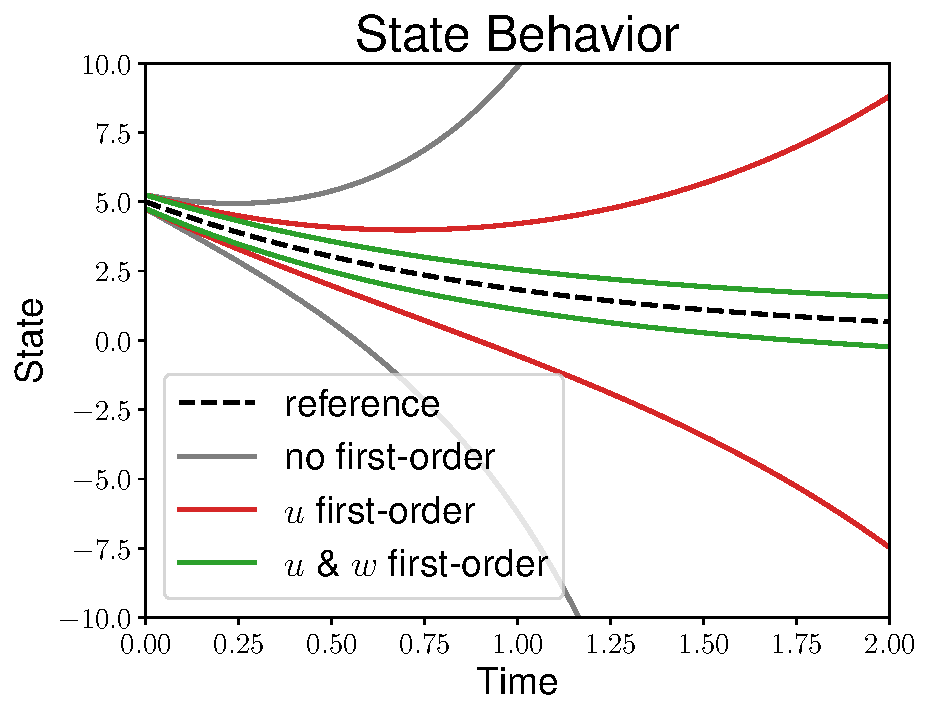
\includegraphics[width=0.75\linewidth]{fig/simplesystem_all3.pdf}
    \caption{Demonstration of the advantages of including first-order interactions of the disturbance in the forward invariant tube calculation. By accounting for these interactions, the tube tightens around the reference trajectory.}
    \label{fig:simple}
\end{figure}

We now provide a simple tutorial example demonstrating the effects of incorporating the first-order interactions of the observed disturbance behavior on the system. We consider the dynamics
\begin{equation}
    \dot{x} = x + u + w
\end{equation}
where the disturbance behavior $w = g(x)$ is dictated by the function $g(x) = -x$. We assume we have estimated disturbance bounds
\begin{align}
    \ul{\gamma}(t, \ul{x}, \ol{x}) &= \min_{x\in[\ul{x}, \ol{x}]}{-x - 1} \\
    \ol{\gamma}(t, \ul{x}, \ol{x}) &= \max_{x\in[\ul{x}, \ol{x}]}{-x + 1}
\end{align}
and known reference controller behavior $u_r = -x$ as well as feedback controller behavior $u = -(x - x_r) + u_r$. We initialize the system at $x = 5$ and then craft several embedding systems: one without modeling first-order disturbance interactions (i.e.~\eqref{eq:init_mixed_emb_lower}--\eqref{eq:init_mixed_emb_upper}), one modeling only the first-order interactions between the input and state (i.e.~\eqref{eq:K_mixed_emb_lower}--\eqref{eq:K_mixed_emb_upper}), and one modeling all first-order interactions (i.e.~\eqref{eq:final_mixed_emb_lower}--\eqref{eq:final_mixed_emb_upper}). We initialize both embedding systems at $[x, \widehat{x}] = [4.75, 5.25]$ and simulate a $2$ second trajectory. As shown in Figure~\ref{fig:simple}, by accounting for the first-order interactions between the disturbance behavior and the system, the forward invariant tube remains tight around the reference trajectory, rather than quickly expanding.
% \sam{We spent too much time on this for it to be subsection 2 of a Case studies section after subsection 1 that is just a toy example...}

% \subsubsection{A Note on Sampling Methods for Deriving $\ul{\gamma}, \ol{\gamma}$}
% As we utilize \acp{GP} in order to model the unknown dynamics, in order to obtain the bounding functions $\ul{\gamma}, \ol{\gamma}$, we employ a sampling-based method. Specifically, we generate a grid of points $x_{g1}, x_{g2}, ...\in[\ul{x}, \ol{x}]$

% thus we must preserve the guarantee via...$[M_s]$


\subsection{Trajectory Tracking Runtime Assurance}
We insert the forward invariant tube formulation outlined in previous sections into the runtime assurance algorithm introduced in~\cite{caoICRARTA}. If it does not hold that
\begin{equation}
    \bigwedge_{i = 1}^{n} |\ul{x}_i(t) - x_{ri}(t)| \leq \varepsilon \wedge |\ol{x}_i(t) - x_{ri}(t)| \leq \varepsilon
\end{equation}
for all $t \geq 0$, then an observation of the unknown disturbance behavior $g(t, x)$ is triggered at the time $t_r$ where
\begin{equation}
    t_r = \min_{t \geq 0} |\ul{x}_i(t) - x_{ri}(t)| \geq \varepsilon \vee |\ol{x}_i(t) - x_{ri}(t)| \geq \varepsilon,
    \label{eq:t_r}
\end{equation}
after which a new reference trajectory is generated. Subsequently, a new feedback term $K$ is computed via solving for a Linear Quadratic Regulator of the system linearized around the current state, along with the resulting forward invariant tube. The overall runtime assurance mechanism is outlined in Algorithm~\ref{alg:mechanism}. 

\begin{algorithm}
\caption{Runtime Assurance Mechanism}
\label{alg:mechanism}
\begin{algorithmic}[1]
\State\algorithmicKwData{Embedding system~\eqref{eq:final_mixed_emb_lower}--\eqref{eq:final_mixed_emb_upper}, safety threshold $\varepsilon$
}

\State$t_r \gets 0$
\While{In Operation}
\If{$t \geq t_r$}
\State $K \gets$ Solution to LQR of~\eqref{eq:system} linearized at x(t)
\State Generate Reference Trajectories $x_r, u_r$ which solve~\eqref{eq:system} for $w_r = \widetilde{\mu}_t(x_r)$, $x_r(t) = x(t)$;
\State $\ul{x}, \ol{x} \gets$ solution to embedding system dynamics~\eqref{eq:final_mixed_emb_lower}--\eqref{eq:final_mixed_emb_upper}, initialized from $\ul{x}(t) = \ol{x}(t) = x(t)$;
\State $t_r \gets \min_{t \geq 0} |\ul{x}_i(t) - x_{ri}(t)| \geq \varepsilon \vee |\ol{x}_i(t) - x_{ri}(t)| \geq \varepsilon$;

\EndIf
\State Apply $u = K(x - x_r) + u_r$;
\EndWhile

\end{algorithmic}
\end{algorithm}

This brings us to the main theoretical result of this work.
\begin{theorem}
    % \michael{TODO: Given Assumption X (which states that there exists some underlying mechanism for producing reference trajectories that satisfy some optimal control requirement), the RTA formulation Algorithm 1 guarantees fulfillment}
    Given reference trajectories $x_r(t), u_r(t)$ provided via Assumption~\ref{assum:refs} that solve~\eqref{eq:system} for $w_r(t) = \widetilde{\mu}_t(x_r(t))$, applying the runtime assurance mechanism outlined by Algorithm~\ref{alg:mechanism} guarantees that no state in the system deviates from the reference trajectory by more than $\varepsilon$ for all $t > 0$.
\end{theorem}
\begin{proof}
    The proof is similar to that of~\cite[Theorem 1]{caoICRARTA}. At the instant $t=t_r$, the reference trajectory is calculated with $x_r(t) = x(t)$ and the tube is initialized with $\ul{x}(t) = \ol{x}(t) = x(t)$. Thus, it must always hold that the next $t_r > t$ given $\varepsilon > 0$ and condition~\eqref{eq:t_r}. Consequently, we can say that $t \leq t_r$ for all $t > 0$ at runtime. 
    
    Per Proposition~\ref{prop:1}, the tube defined by $[\ul{x}(t), \ol{x}(t)]$ is such that, for all $t \geq 0$, applying the control strategy outlined by Algorithm~\ref{alg:mechanism} results in $x(t) \in [\ul{x}(t), \ol{x}(t)]$. Thus, combining Propsition~\ref{prop:1} with condition~\eqref{eq:t_r} results in
    \begin{equation}
        x(t) \in [\ul{x}(t), \ol{x}(t)] \subseteq [x_r(t) - \varepsilon, x_r(t) + \varepsilon]
    \end{equation}
    for all $t < t_r$. Since $t < t_r$ for all time, it must hold that
    \begin{equation}
        x(t) \in [x_r(t) - \varepsilon, x_r(t) + \varepsilon]\ \forall_{t > 0}
    \end{equation}
\end{proof}
Thus, Algorithm~\ref{alg:mechanism} solves Subproblem~\ref{prob:rta}. Combined with a reference trajectory generator that satisfies Assumption~\ref{assum:refs}, the overall runtime assurance mechanism solves our overall problem statement.
In the next sections, 
% we provide a method for deriving an optimal feedback term $K$, 
we demonstrate a simple numerical example showcasing the benefits of directly incorporating the first-order interactions of the disturbance behavior, and then implement our forward invariant tube formulation on a planar multirotor system, first in simulation and subsequently on a software-in-the-loop setup.

% \subsection{Feedback Controller Synthesis}
% % we can put in the controller synthesis stuff here but it does worse than just doing LQR on the linearization of the system around the current state when doing the recalculation of trajectories
% % this result makes sense but how to sell it?
% % at minimum we can just do it with LQR

% While a predetermined feedback term $K$ can be used in~\eqref{eq:feedback_controller} and the resulting equation~\eqref{eq:final_inc} to produce a valid embedding system, we now provide a formulation for synthesizing a feedback term $K$ via optimization over a Linear Matrix Inequality formed from an initial open-loop tube computed around the reference trajectory. This $K$ is guaranteed to be...

% We first compute...
% \begin{equation}
%     \begin{bmatrix}[\mathcal{M}_x] + [\mathcal{M}_w][\mathcal{M}_g]\end{bmatrix}
%     \label{eq:Ainterval}
% \end{equation}

% We then adapt from~\cite{lmibook}
% \begin{equation}
%     \begin{bmatrix}
%         AQ+QA^T+BY+Y^TB^T & (CQ+DY)^T\\
%         CQ+DY & -I
%     \end{bmatrix} < 0
%     \label{eq:lmi}
% \end{equation}

% and insert the corners of~\eqref{eq:Ainterval} into $A$, while defining $B := $, $C := $, and $D:= $.

% We then form the optimization problem
% \begin{align}
%  \underset{Y, Q}{\text{minimize}} & \text{ trace}(Q) \label{eq:optimization}\\
%  \text{subject to:}\hspace{5pt}&\nonumber \\
%  &\hspace{-40pt} \eqref{eq:newlmi}\nonumber
% \end{align}

% Finally, we take the solved $Y, Q$ and derive the resulting feedback controller term $K$ via
% \begin{equation}
%     K = YQ^{-1}
%     \label{eq:K}
% \end{equation}

% \begin{theorem}
%     The feedback term $K$ as computed by~\eqref{eq:K} minimizes...
% \end{theorem}

% \sam{We don't have a theorem? The punchline should be clearer with more narrative, etc.}

\section{Case Studies}
\label{section:sim}
In this section we provide demonstrations of our forward invariant tube formulation in various applications. We first showcase the formulation on a five-dimensional planar multirotor example via a trajectory tracking scenario in simulation, before demonstrating the formulation on a software-in-the-loop setup in order to both showcase its computational viability for deployment on physical hardware and demonstrate its capabilities in conditions more extreme than can be produced in a controlled environment. Finally, we showcase the assurance mechanism running on a physical multirotor.\footnote{Code for these case studies can be found at \url{https://www.github.com/gtfactslab/TODO}}

\subsection{Simulation}
\begin{figure}[t!]
\centering
  
  \begin{tikzpicture}
    \begin{axis}[width=1in,
    axis y line=middle,
    axis x line=middle,
every axis x label/.style={at={(current axis.right of origin)},anchor=west},
   xmin=0, xmax=2, ymax=-1.5,ymin=0, ytick=\empty, xtick=\empty,xticklabel={$-\frac{b}{M}$}, yticklabel style={anchor=west},
   xlabel style={anchor=north},
   ylabel style={anchor=south east},
    xlabel={$y$},
    ylabel={$z$},
    x=1cm,y=1cm, 
    disabledatascaling,
    clip=false
    ]
    \addplot[mblue, line width=1pt] file {quad.txt};
    \draw[dashed] (0,0) -- +(20:1.8);
    \draw[->] (1.5,0) arc (0:20:1.5) node[right, pos=.5] {$\theta$};
    \draw[->, line width=1pt, draw=gray] (0,0) -- node[left,pos=1]{$u_1$}+(110:.8);
    \draw[->, line width=1pt, draw=gray] (20:.2) arc (20:310:.2) node[below,pos=.8] {$u_2$};
    \draw[->, dashed] (1.4,0.5) -- node[right,pos=1]{}+(20:.8);
    % \draw[->, dashed] (1.4,0.5) -- node[left,pos=1]{$v$}+(110:.8);
%    \node at (1.8,.7) {$(y,z)$};
  %  \node [circle, fill=blue, inner sep=1pt] at (1.3,1) {};
  \end{axis}

  \end{tikzpicture}
  \caption{The planar multirotor model has horizontal position $y$, vertical position $z$, and roll angle $\theta$. The inputs are thrust $u_1$ in the direction perpendicular to the line segment connecting the rotors and roll angle acceleration $u_2$.}
  \label{fig:quad}
\end{figure}

\begin{figure}
    \centering
    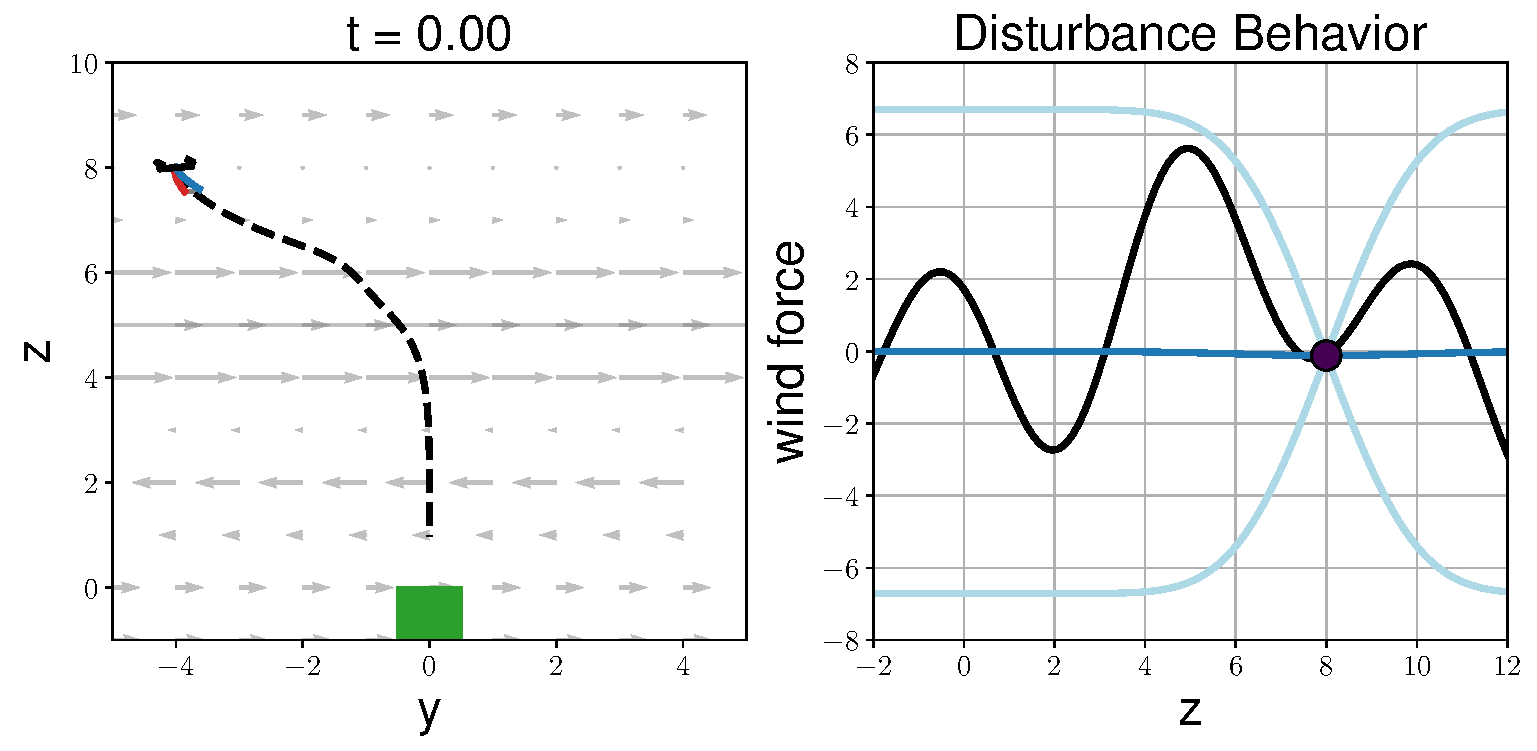
\includegraphics[width=0.95\linewidth]{fig/rta_nosynth_0.00.pdf}
    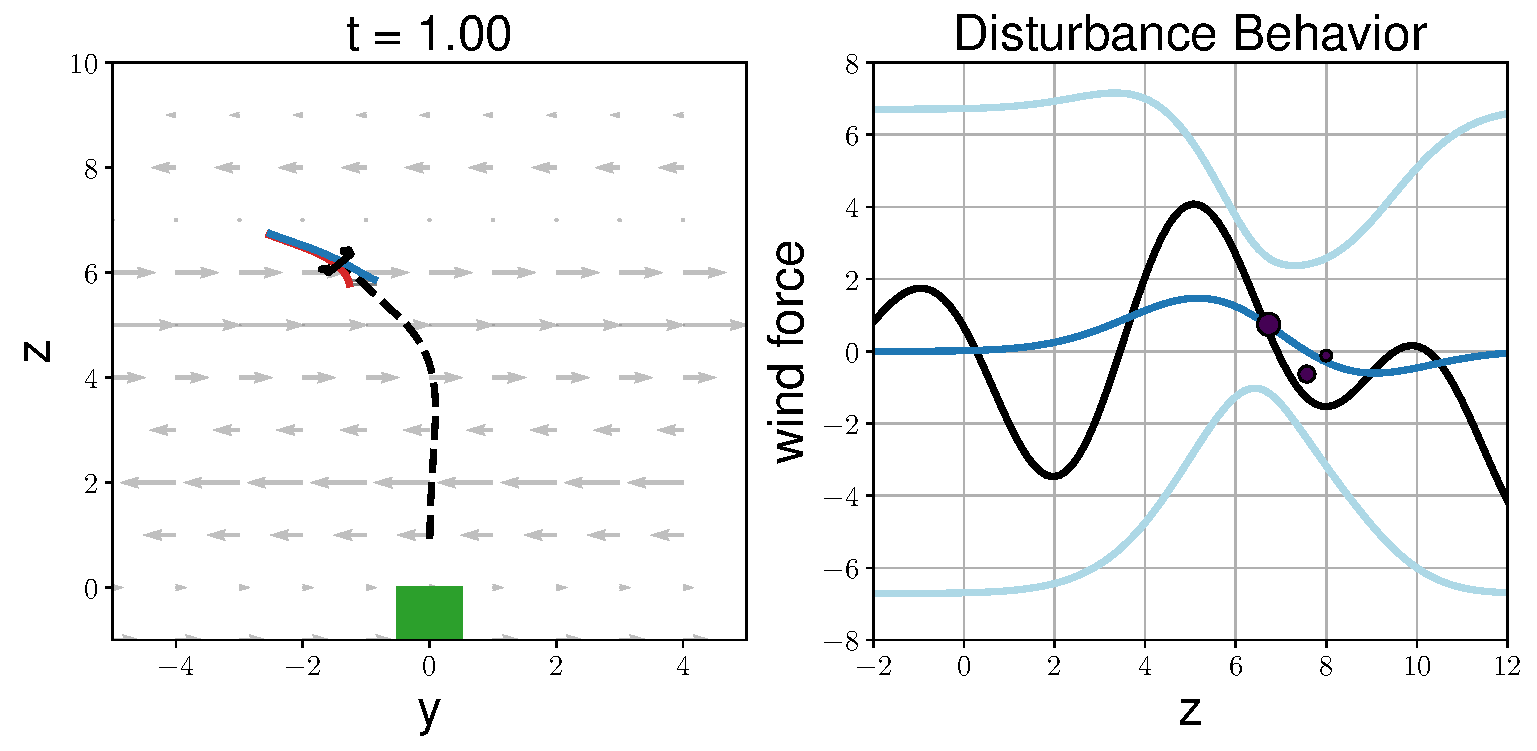
\includegraphics[width=0.95\linewidth]{fig/rta_nosynth_1.00.pdf}
    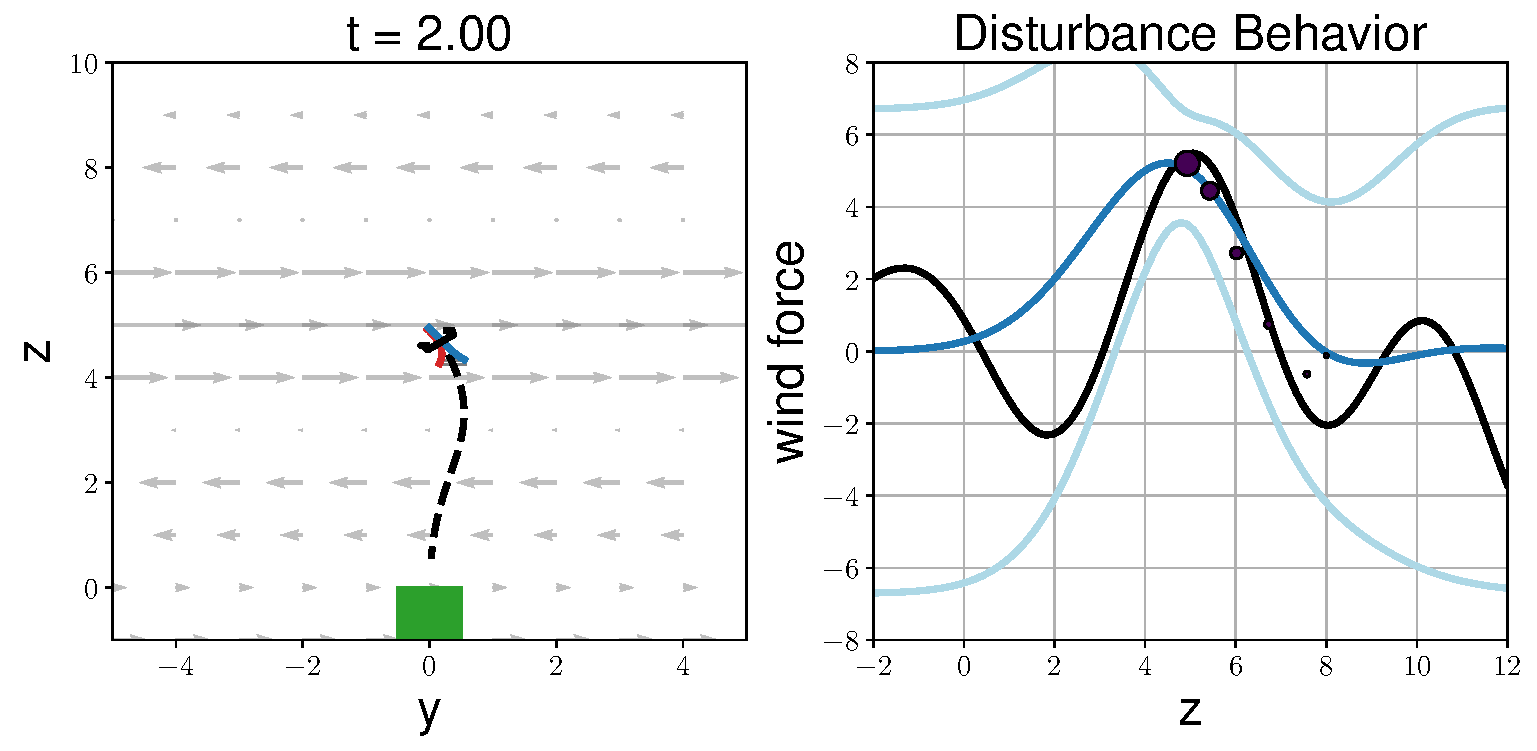
\includegraphics[width=0.95\linewidth]{fig/rta_nosynth_2.00.pdf}
    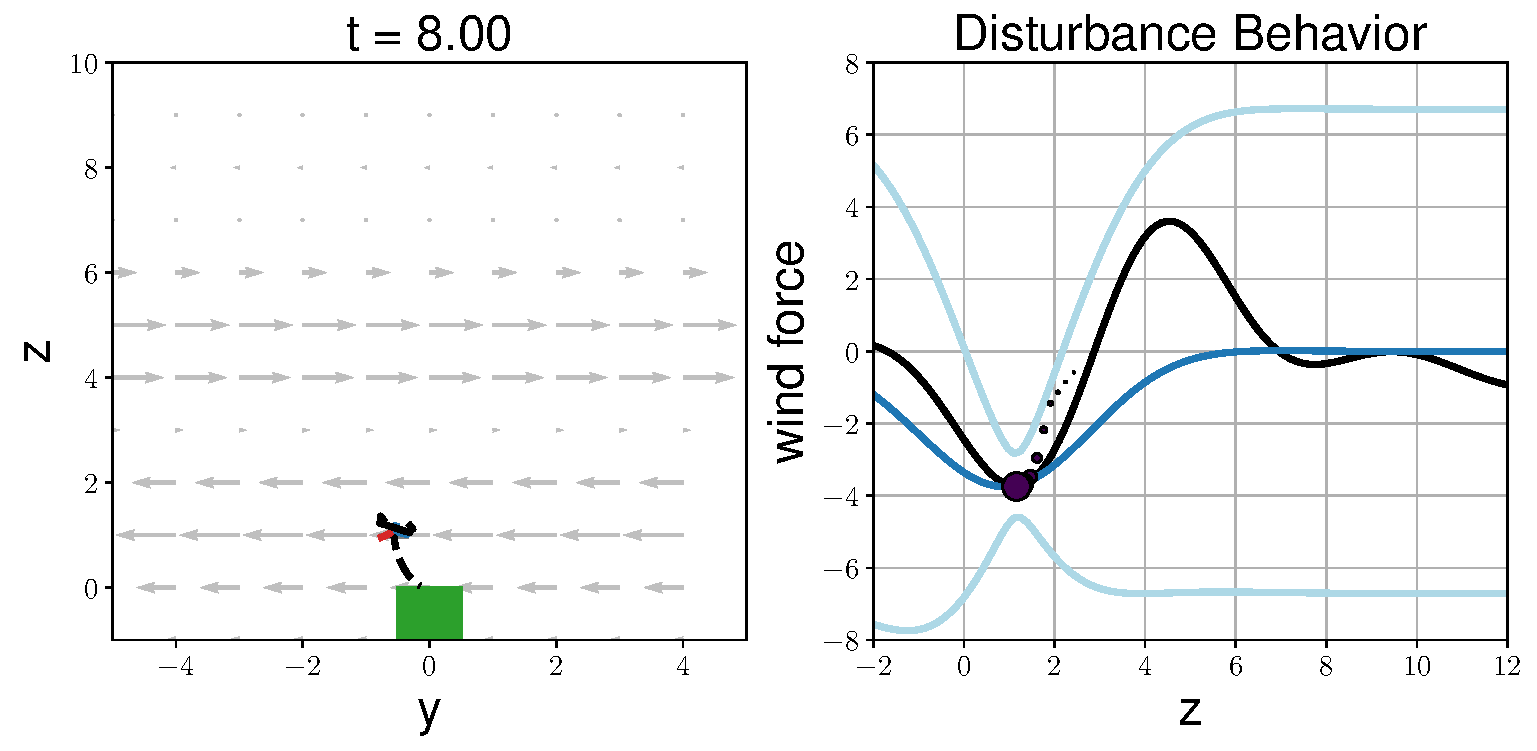
\includegraphics[width=0.95\linewidth]{fig/rta_nosynth_8.00.pdf}
    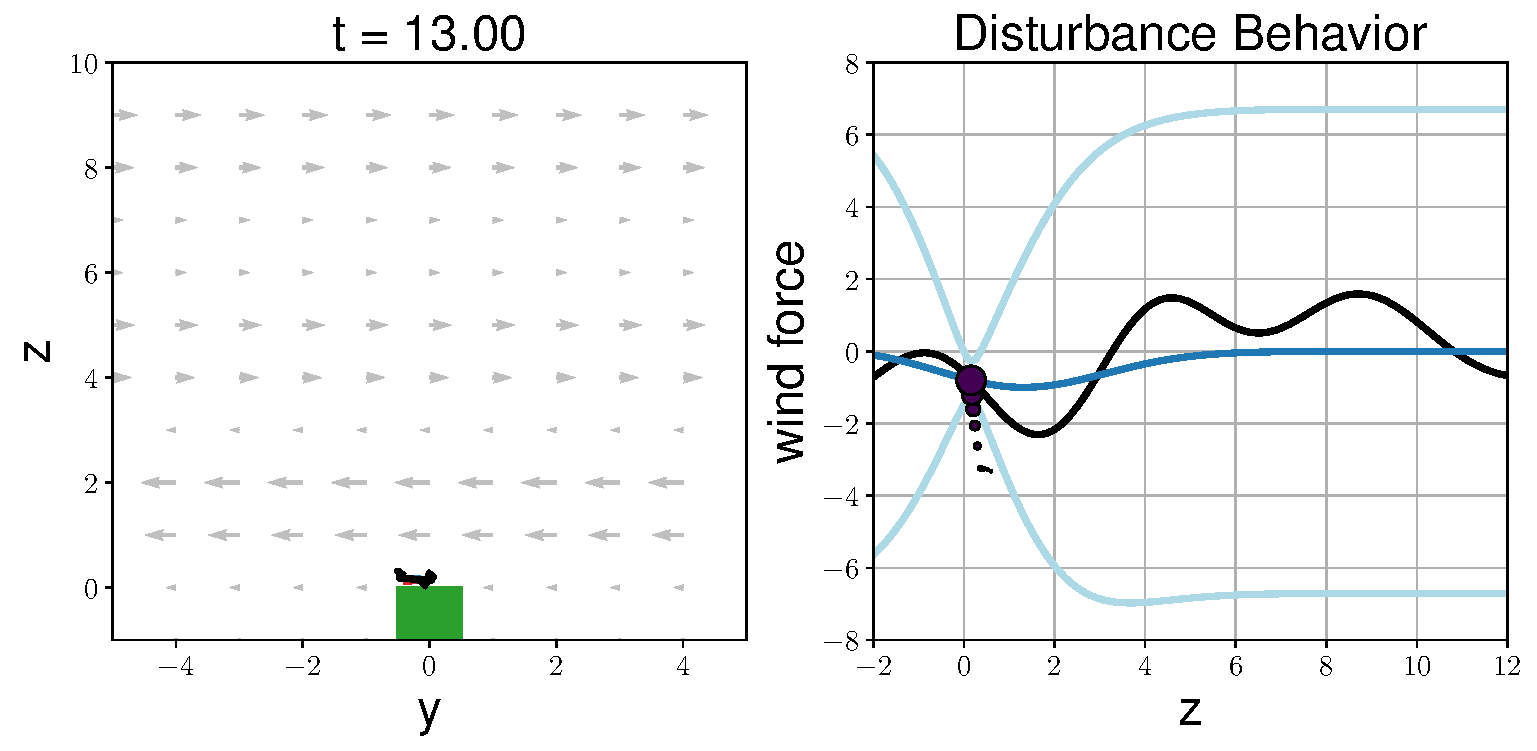
\includegraphics[width=0.95\linewidth]{fig/rta_nosynth_13.00.pdf}
    \caption{The planar multirotor trajectory tracking simulation. The multirotor attempts to track a landing reference trajectory (left, dashed), while the runtime assurance algorithm calculates a forward invariant tube (left, red and blue) using observations (right, dots, largest most recent) to estimate the mean and confidence bounds (right, dark and light blue respectively) on the disturbance (right, solid black). Per Algorithm~\ref{alg:mechanism}, an observation is collected and the trajectories are recomputed whenever the forward invariant tube deviates from the reference beyond the safety threshold.}
    \label{fig:rta}
\end{figure}

We now consider a multirotor system constrained to moving within the vertical plane, and apply our forward invariant tube calculation to the runtime assurance mechanism outlined in~\cite{caoICRARTA}. The five-dimensional state $x$ of the planar multirotor system consists of horizontal position $y$, vertical position $z$, roll angle $\theta$, and the derivatives $\dot{y}$ and $\dot{z}$, so that $x=\begin{bmatrix}y\ \dot{y}\ z\ \dot{z}\ \theta\end{bmatrix}^T$. The two inputs are thrust $u_1$  acting at the center of mass in the direction $\begin{bmatrix}-\sin\theta&\cos\theta\end{bmatrix}^T$ perpendicular to the line segment connecting the rotors, and roll angular velocity $u_2$. Additionally, there exists a time and altitude-dependent wind force $g(t, z)$ acting horizontally which is unknown a priori. Thus, the normalized dynamics of the system are
\begin{equation}
  \label{eq:planarquad}
  \begin{split}
  \ddot{y}&=-u_1\sin \theta+g(t, z)\\
  \ddot{z}&=u_1\cos \theta-a_g\\
  \dot{\theta}&=u_2
  \end{split}
\end{equation}

We then implement the runtime assurance algorithm outlined in Algorithm~\ref{alg:mechanism}. We first generate a reference trajectory by linearizing the system~\eqref{eq:planarquad} around the equilibrium and then employing a Linear-Quadratic Regulator (LQR) feedback controller with parameters
$Q = \text{diag}([1000, 500, 20, 500, 1])$ and $R = \text{diag}([20, 20])$ to simulate a trajectory to the origin assuming $g(t, z) = \widetilde{\mu}_t(z_r)$. The resulting state and input trajectories form the reference trajectories $x_r, u_r$ that we use to calculate the forward invariant tube.

We designate a safe landing hyperrectangle $\mathcal{X}_\text{land} := [(-0.5, -0.1, -1, -0.1, -\pi/6), (-0.5, 0.1, 0, 0.1, \pi/6)]$ and then calculate the forward invariant tube of the system using the embedding system~\eqref{eq:final_mixed_emb_lower}--\eqref{eq:final_mixed_emb_upper} and the current estimated $\widetilde{\mu}_t, \widetilde{\sigma}_t$. We apply the control strategy~\eqref{eq:feedback_controller} and calculate the future time $t_r$ at which any state deviates beyond the reference trajectory by $\varepsilon$ or more. At that time, we collect an observation of the disturbance behavior and recalculate the reference trajectory and forward invariant tube. This guarantees that the system remains within $\varepsilon$ of the reference trajectory for all time. The overall runtime assurance mechanism is outlined in Algorithm~\ref{alg:mechanism}.





As shown in Figure~\ref{fig:rta}, the multirotor is initially unable to guarantee a safe landing as the forward invariant tube quickly expands past the allowed threshold. As the quadcopter descends, we collect observations and update the reference trajectory and forward invariant tube, taking into account the time at which each observation was taken and weighting them appropriately in the confidence bounds on the disturbance behavior. The multirotor is eventually able to achieve a safe landing even in the presence of this time-varying disturbance behavior. Additionally, with the exact same safety parameters, we note that the average computed $t_r$ was $0.21$ seconds without accounting for the first-order interactions between the disturbance and state, and $0.38$ seconds with them, which illustrates the benefits of including said first-order interactions in tightening the forward invariant tube.
We implemented this simulation on a personal computer with the \texttt{immrax} library~\cite{immrax}. 
% Calculating the reference trajectories and the forward invariant tube takes approximately $0.04$ seconds, and a recalculation is triggered approximately every $0.3$-$1.0$ seconds, showcasing the real-time capabilities of the formulation.

% \subsection{Implicit Active Set Invariance Filtering}
% \begin{figure}
%     \centering
%     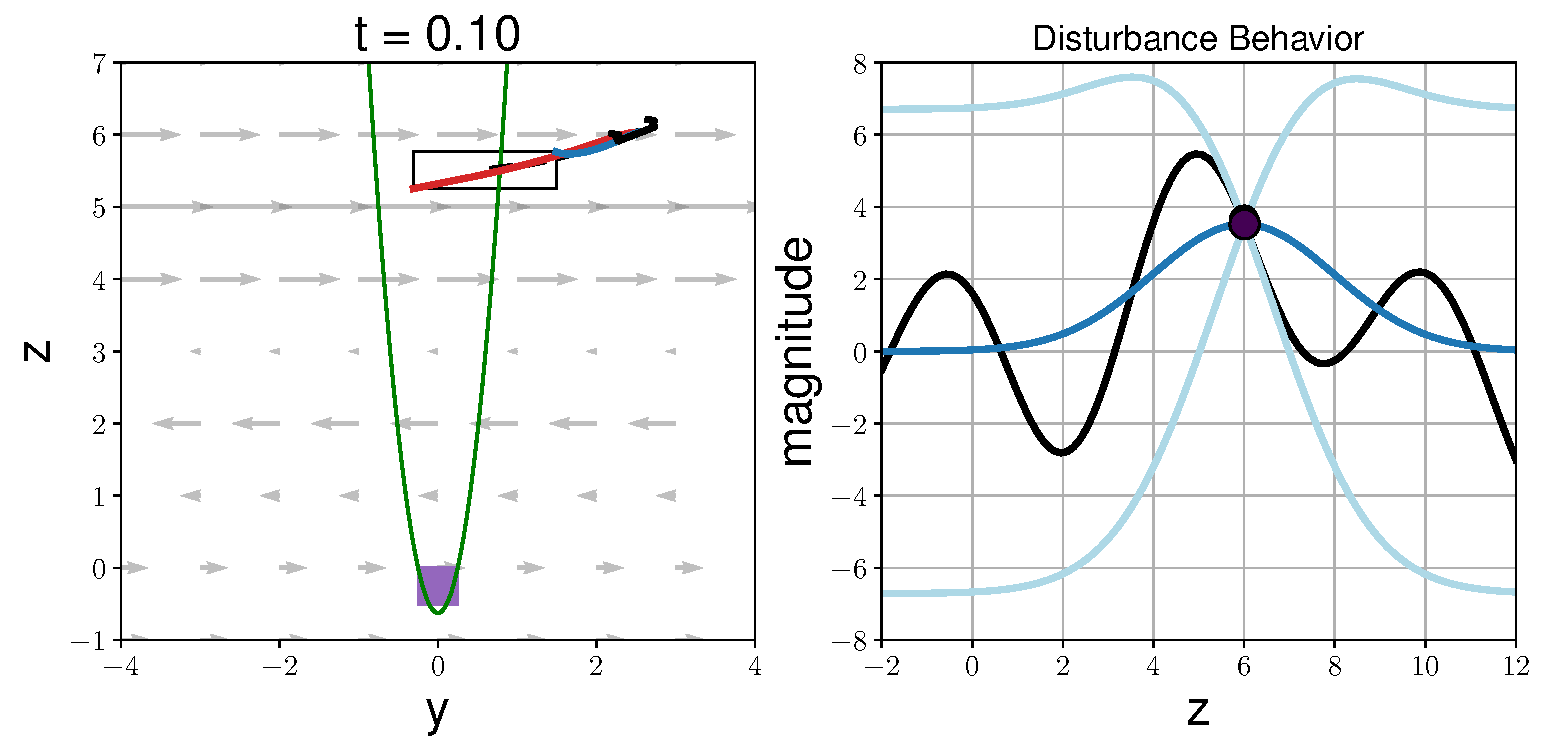
\includegraphics[width=0.45\linewidth]{fig/iasif_0.10.pdf}
%     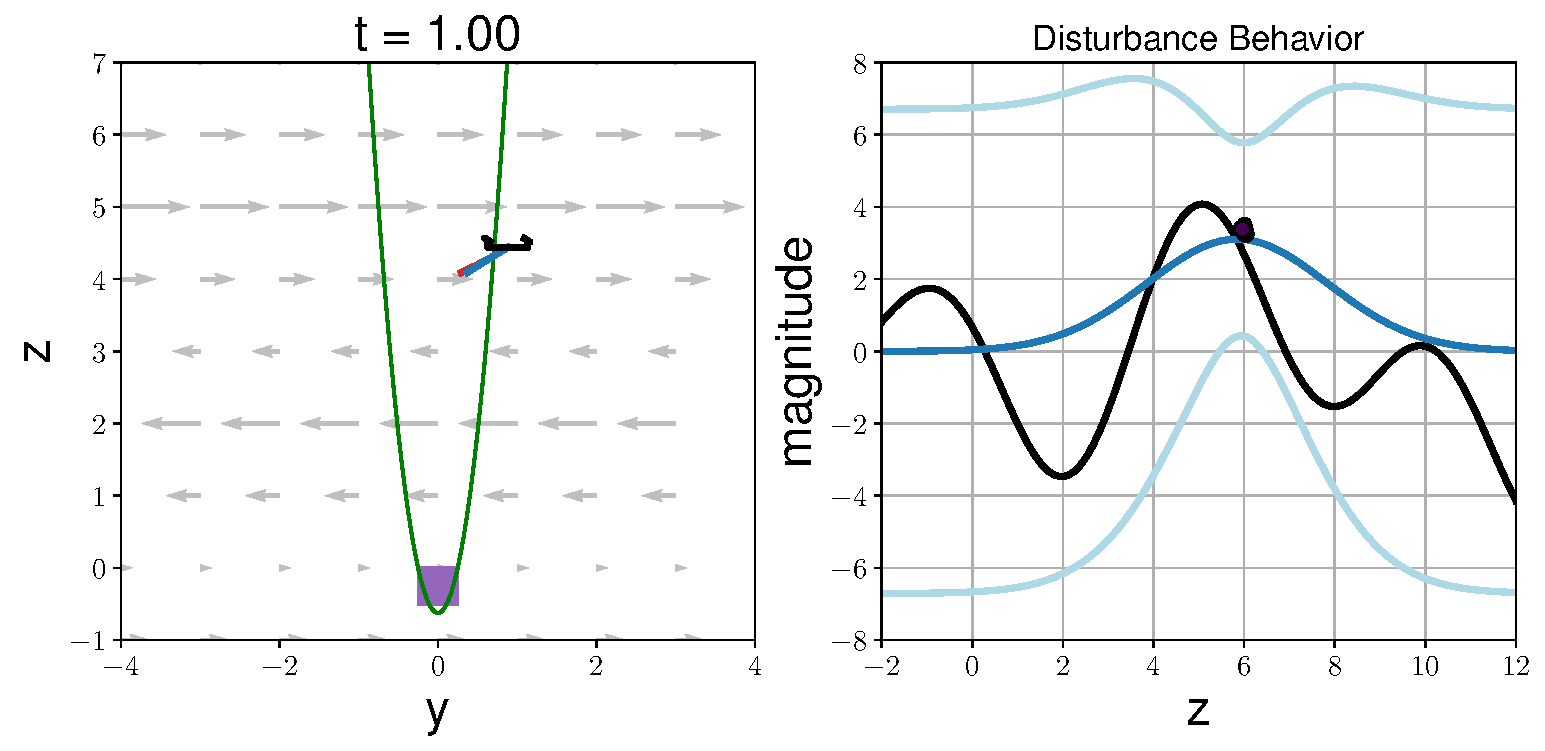
\includegraphics[width=0.45\linewidth]{fig/iasif_1.00.pdf}
%     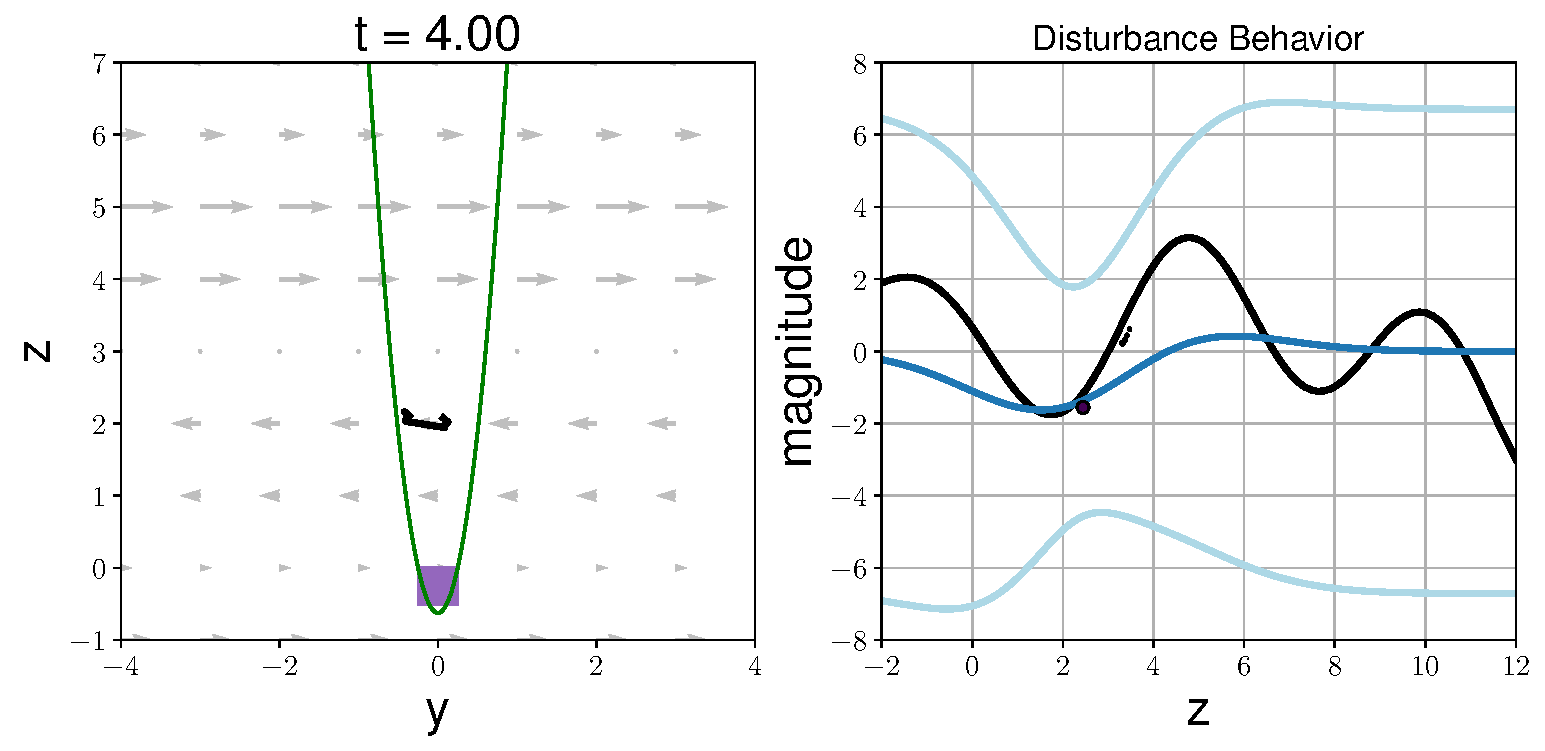
\includegraphics[width=0.45\linewidth]{fig/iasif_4.00.pdf}
%     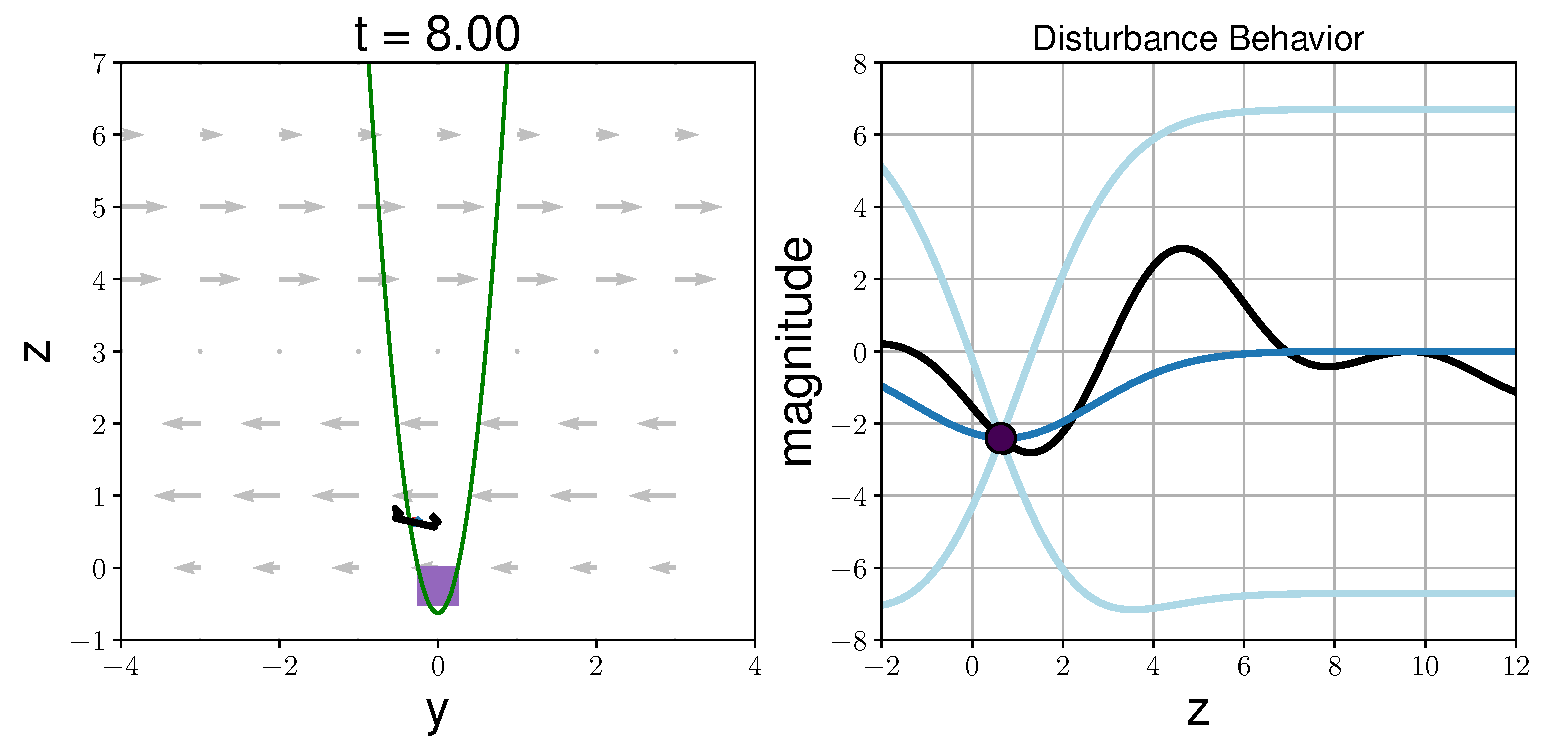
\includegraphics[width=0.45\linewidth]{fig/iasif_8.00.pdf}
%     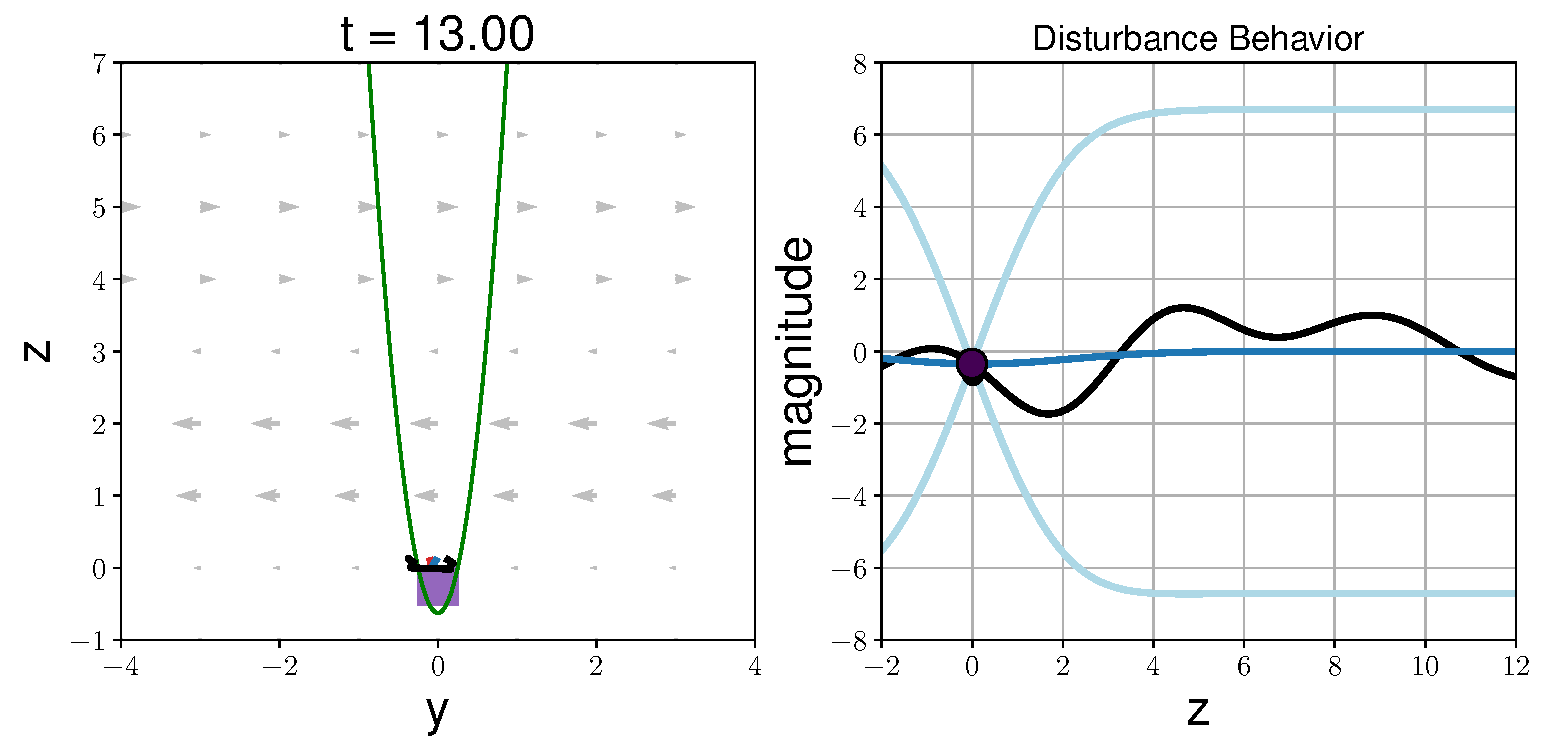
\includegraphics[width=0.45\linewidth]{fig/iasif_13.00.pdf}
%     \caption{The planar multirotor Implicit ASIF simulation. The multirotor attempts to land via an uncertified controller. At all times, the filter calculates the least intrusive modification to the desired input such that a backup trajectory (left, red and blue) back to the safety region (left, green) always exists. The formulation incorporates observations (right, dots, largest most recent) to estimate the mean and confidence bounds (right, dark and light blue respectively) on the disturbance (right, solid black), which are collected whenever no part of the forward invariant tube fully fits within the safety region.}
%     \label{fig:iasif}
% \end{figure}

% We now consider a scenario in which a separate, unverified control strategy is developed for landing, and insert our trajectory tracking formulation into an Implicit Active Set Invariance Filtering formulation to act as a safety filter for said controller. We define a function $h(x)$ and a resulting safety set $\mathcal{S}$ such that
% \begin{equation}
%     \mathcal{S}:= \{x \in \mathbb{R}^n | h(x) \geq 0\},
% \end{equation}
% which, for this case study, is defined as
% \begin{equation}
%     h(x) := -(10(y^2 - 0.0625) - z)
% \end{equation}
% which produces the region outlined in green in Figure~\ref{fig:iasif}.

% We then implement an Implicit Active Set Invariance Filter (see, e.g.,~\cite{llanesIASIF}), which minimally perturbs the desired input such that a backup trajectory that drives the system into $\mathcal{S}$ always exists. Our embedding system formulation~\eqref{eq:final_inc} produces the backup trajectory and forward invariant tube used in the filter. As shown in Figure~\ref{fig:iasif}, when there is no guaranteed path back to the safety set (i.e., no slice of the forward invariant tube is fully contained in the safety set), an observation is taken and the filter steps in and drives the system with the maximum force back toward it. This continues until a safe landing is achieved. The filter takes around $0.01$ seconds to compute on average, showcasing its capabilities for real-time computation.

\subsection{Software-in-the-Loop Demonstration}
To demonstrate the viability of our formulation on hardware, we validate Algorithm \ref{alg:mechanism} using a PX4 Autopilot~\cite{PX4} software-in-the-loop (SITL) simulation in the Gazebo simulator~\cite{Gazebo}. 
% This software in the loop simulation goes beyond traditional simulation avenues like numerical simulators or more advanced simulators such as MuJoCo and PyBullet. Because 
Unlike numerical simulators such as MuJoCo or PyBullet—which only integrate rigid-body dynamics—SITL runs the exact same PX4 firmware used on physical flight controllers, with no modifications or simplifications. All estimation, control, motor-mixing, and safety checks execute in real time exactly as they would on embedded hardware.

Gazebo complements this by providing a hardware-realistic sensor stack (IMU, magnetometer, barometer, GPS, cameras, etc), complete with sensor noise, latency, and their own update rates, as well as actuator dynamics, aerodynamic disturbances, and asynchronous ROS 2 communication. All of this makes PX4 SITL in Gazebo fundamentally different from and substantially more realistic than physics-only simulators. Consistent with prior experience of the authors, controllers that perform reliably in this SITL environment generally transfer to hardware deployment with minimal modifications needed to accommodate safety and system modeling.

To preserve computational tractability and maintain parallel development, we retain the planar quadrotor assumption. However, we extend the formulation to include wind disturbances in both the horizontal and vertical directions in order to capture coupled airflow effects that may be encountered in hardware testing environments (e.g., laboratory experiments employing high-power industrial fans oriented diagonally to generate sustained wind disturbances). Notably, a key strength of the Gazebo software-in-the-loop (SITL) framework is its ability to impose much harsher wind conditions than can be realized in laboratory-scale experimental setups. With simulated wind speeds averaging \qty{17}{m/s}, realistic physics and sensor modeling, and the same flight stack used on hardware platforms, the SITL framework enables high-fidelity evaluation of the performance of our proposed method under near gale-force landing conditions.

Utilizing a North-East-Down coordinate frame and non-unit mass, the dynamics of the planar quadrotor system become
\begin{equation}
  \label{eq:planarquad_hardware}
  \begin{split}
  \ddot{y}&=u_1\sin \theta + \frac{g_y(t, z)}{m}\\
  \ddot{z}&=-u_1\cos \theta + a_g - \frac{g_z(t,y)}{m}\\
  \dot{\theta}&=u_2.
  \end{split}
\end{equation}

However, these dynamics will only hold if the true quadrotor behaves approximately as a planar system. The true system takes a full input vector \(u = \begin{bmatrix}u_1, u_2, u_3, u_4\end{bmatrix}^\top \in \mathbb{R}^4\), where \(u_3\) and \(u_4\) are pitch and yaw angular body rates. In order to ensure that the runtime assurance mechanism interacts with a system constrained to movement within the vertical plane, we employ a joint control strategy to calculate \(u_3\) and \(u_4\) separately from \(u_1\) and \(u_2\) to maintain a constant yaw and \(x\) position of zero. In our case, we utilize the Newton Raphson-based control strategy~\cite{Wardi-NR}, which is computationally efficient while providing accurate tracking in quadrotor hardware experiments~\cite{Evanns-NR}. In addition, we regularly re-linearize and re-compute the LQR gain to achieve stable tracking of the runtime assurance reference trajectory by \(u_1\) and \(u_2\) .

We note that when controlling body rates directly, new control inputs must be published to the quadrotor at an average of \qty{100}{Hz} in order to achieve flight stability and reduce the risk of crash-landings in both SITL and hardware implementations. This means that the entirety of Algorithm~\ref{alg:mechanism}, the Newton-Raphson controller, and re-calculating the entire LQR pipeline must take at worst \qty{10}{ms} on average to avoid the risk of catastrophic results.

As Table~\ref{tab:computation_times} shows, solving~\eqref{eq:final_mixed_emb_lower}--\eqref{eq:final_mixed_emb_upper} may by itself take as long as \qty{10}{ms}. However, it does not need to be solved at every iteration, only when \(t \geq t_r\). Over the course of the entire SITL experiment, this occurred 82 times. For reference, computing control inputs occurred 1085 times. Thus, the entire control and runtime assurance pipeline, including computing~\eqref{eq:final_mixed_emb_lower}--\eqref{eq:final_mixed_emb_upper}, took \qty{.009}{s} on average, well within safe limits. We achieve these computation speeds due to the pipeline's implementation with JAX and \texttt{immrax}, enabling just-in-time (JIT) compilation in python for the runtime assurance mechanism and the Newton-Raphson controller.


\begin{table}[t!]
    \centering
    \caption{SITL Computation Time Statistics}
    \label{tab:computation_times}
    \begin{tabular}{l c c}
        \hline
        \textbf{Computation} & \textbf{Average (ms)} & \textbf{Max (ms)} \\
        \hline
        Joint Controller & \(0.0026 \pm 0.00069\) & 0.00677 \\
        Invariant Tube   & \(0.108 \pm 0.0059\)  & 0.134 \\
        \hline
    \end{tabular}
\end{table}


\begin{figure}
    \centering
    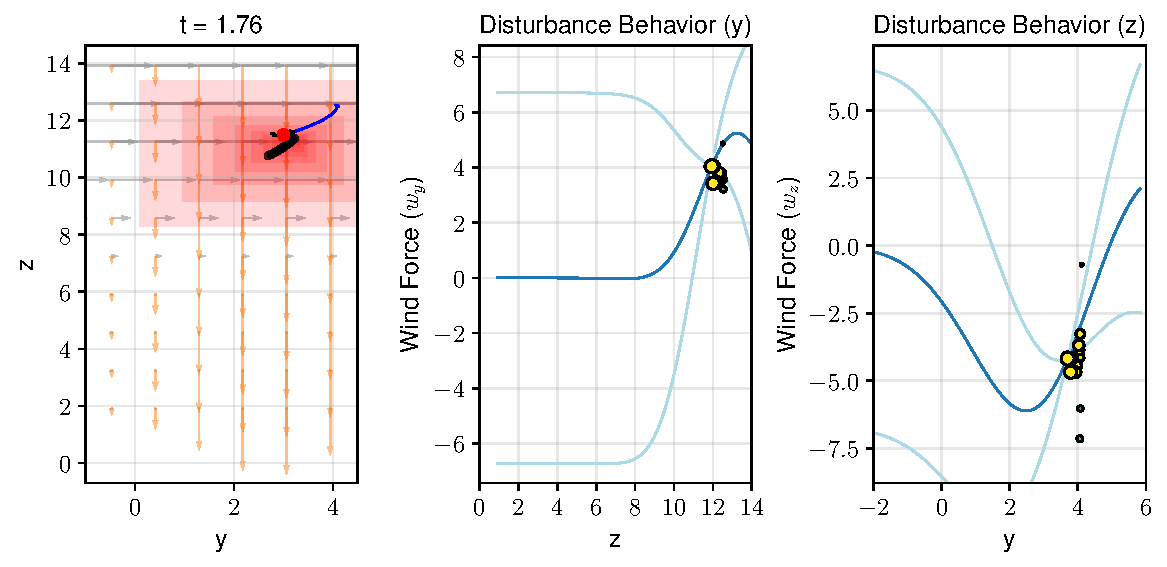
\includegraphics[width=0.95\linewidth]{fig/SITL11.pdf}
    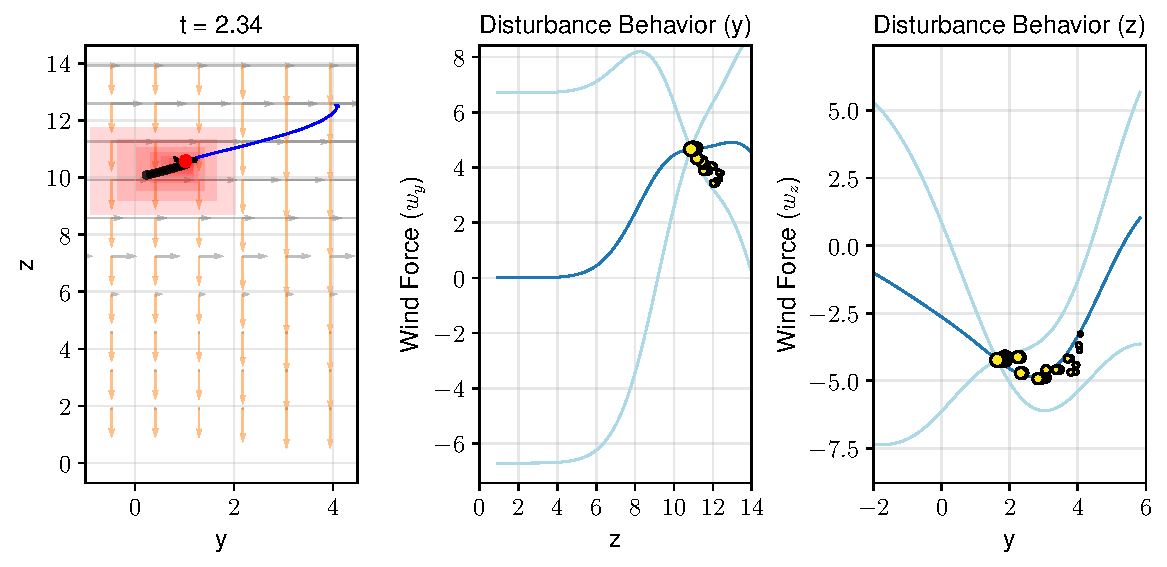
\includegraphics[width=0.95\linewidth]{fig/SITL22.pdf}
    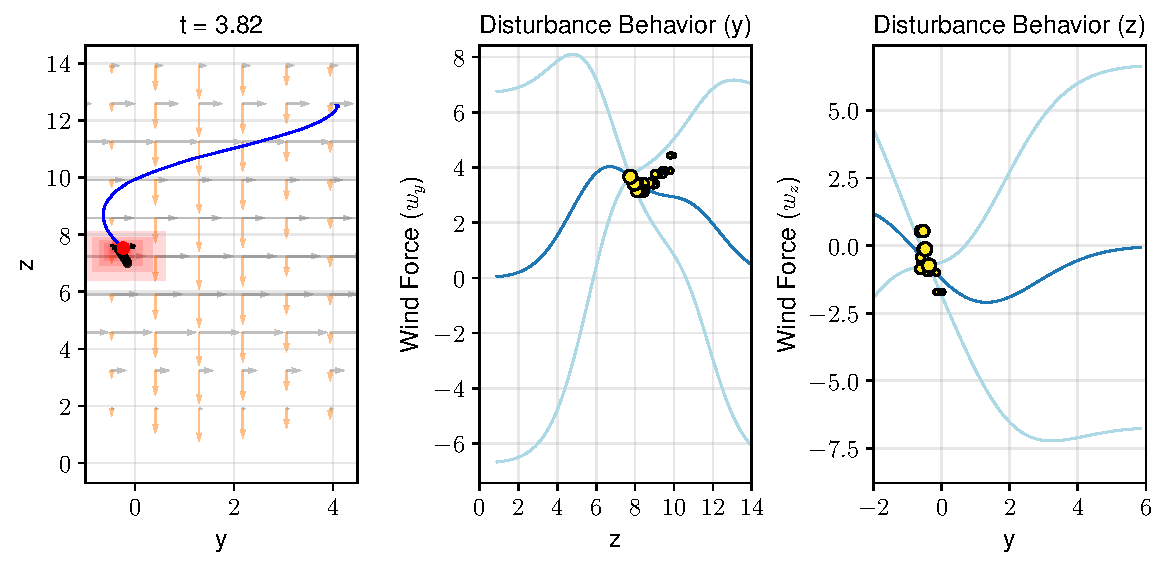
\includegraphics[width=0.95\linewidth]{fig/SITL33.pdf}
    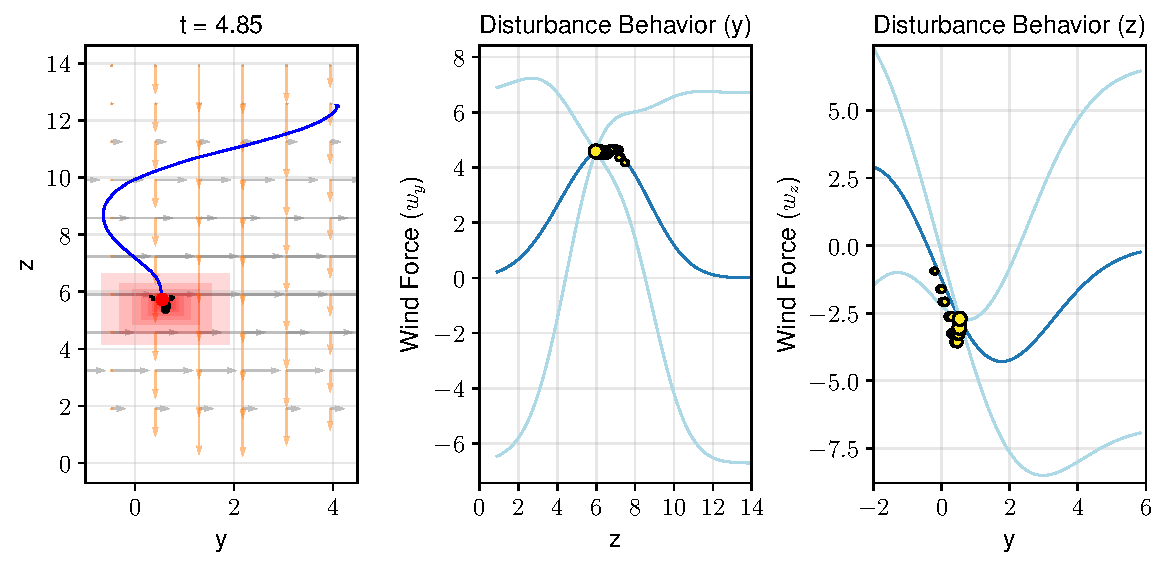
\includegraphics[width=0.95\linewidth]{fig/SITL44.pdf}
    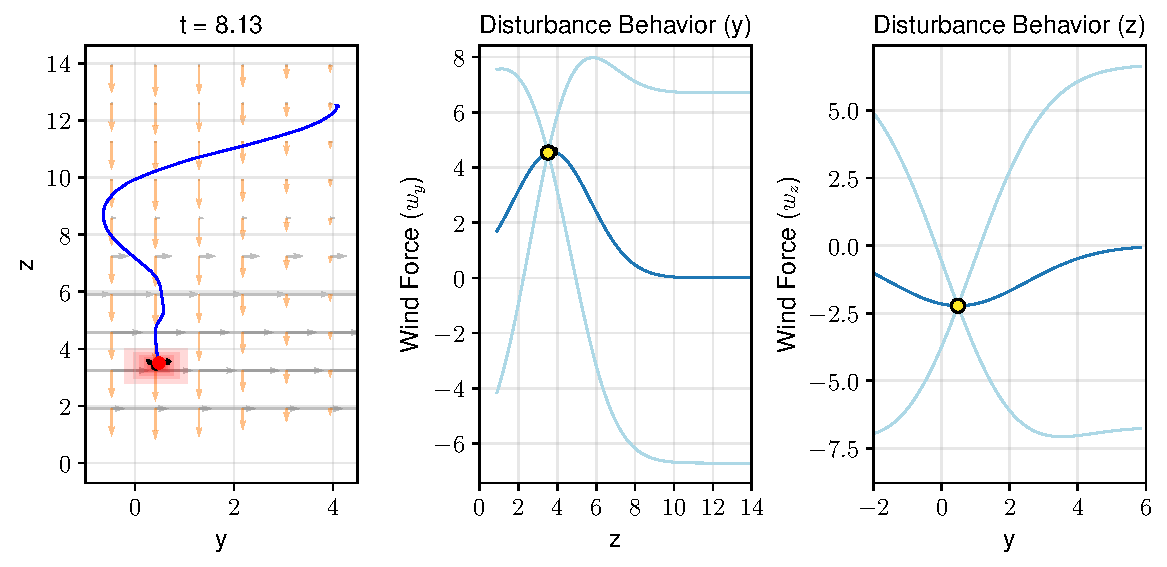
\includegraphics[width=0.95\linewidth]{fig/SITL55.pdf}
    \caption{The software-in-the-loop multirotor trajectory tracking simulation. The multirotor attempts to track the reference trajectory (left, black) while the runtime assurance algorithm produces a forward invariant tube (left, rectangles) using observations (center \& right, dots, largest most recent) to estimate the mean and confidence bounds (center \& right, dark and light blue respectively) on the disturbance, which acts in both the $y$ and $z$ directions, then triggers an observation and recomputation at the appropriate times. The resulting trajectory is on the left in blue.}
    \label{fig:SITL}
\end{figure}

\subsection{Hardware Demonstration}

Having validated Algorithm~\ref{alg:mechanism} under near gale-force conditions in SITL, we now deploy the same pipeline—without modification—on a physical quadrotor platform.\footnote{Full GIF visualizations and hardware video demonstrations can be found at: \texttt{\href{https://github.com/evannsmc/PX4\_RTA\_MM\_GPR/tree/main}{https://github.com/evannsmc/PX4\_RTA\_MM\_GPR/tree/main}}} The hardware experiment is conducted indoors with a high-power fan oriented to produce a sustained lateral wind disturbance. While the fan-induced airflow is considerably milder than the \qty{17}{m/s} simulated winds used in the SITL evaluation, it is sufficient to meaningfully perturb the vehicle throughout the mission and constitutes a genuine, unmodeled real-world disturbance of the form $g(t, z)$ assumed in~\eqref{eq:planarquad_hardware}.

The mission is structured as follows: the quadrotor takes off and flies to an initial position displaced from the origin, holding a brief hover while awaiting the mission start. It then navigates back toward a point above the origin against an a priori unknown wind disturbance, sustaining a hover there for a predetermined period before executing a safe landing. Critically, the fan is positioned adjacent to the origin, so the disturbance grows in magnitude as the vehicle closes on its goal. The reference trajectory $x_r$ is computed via the same LQR-based strategy described in Subsection~\ref{subsec:sim}, with system matrices and LQR gains re-linearized and re-computed at regular intervals along the trajectory.

\begin{figure}[t!]
    \centering
    \includegraphics[width=0.95\linewidth]{fig/hw_yes_wind1.pdf}
    \includegraphics[width=0.95\linewidth]{fig/hw_yes_wind2.pdf}
    \includegraphics[width=0.95\linewidth]{fig/hw_yes_wind3.pdf}
    \includegraphics[width=0.95\linewidth]{fig/hw_yes_wind4.pdf}
    \caption{Hardware experiment with wind estimation enabled. The quadrotor tracks the reference trajectory (left, blue dashed) while the runtime assurance algorithm produces a forward invariant tube (left, red rectangles) using time-weighted observations (center \& right, dots, most recent largest) to estimate the GP mean and confidence bounds (center \& right, dark and light blue) on the horizontal and vertical wind disturbances $g_y(t,z)$ and $g_z(t,y)$ respectively. Wind arrows at the drone indicate the GP-estimated disturbance direction and magnitude at the current state. The drone successfully holds station above the origin and lands safely.}
    \label{fig:hw_yes_wind}
\end{figure}

\begin{figure}[t!]
    \centering
    \includegraphics[width=0.95\linewidth]{fig/hw_no_wind1.pdf}
    \includegraphics[width=0.95\linewidth]{fig/hw_no_wind2.pdf}
    \includegraphics[width=0.95\linewidth]{fig/hw_no_wind3.pdf}
    \includegraphics[width=0.95\linewidth]{fig/hw_no_wind4.pdf}
    \caption{Hardware experiment with wind estimation disabled. Without GP-informed reachable set computations, the runtime assurance mechanism treats the disturbance as zero and the forward invariant tube quickly expands beyond the safety threshold with no corrective observation mechanism. The drone is unable to plan safely against the unmodeled wind and is driven toward the ground, failing to complete the hover-and-land mission.}
    \label{fig:hw_no_wind}
\end{figure}

As Figure~\ref{fig:hw_yes_wind} shows, when wind estimation is enabled, the drone continuously collects disturbance observations and updates the TV-GP estimate of $g_y(t,z)$ and $g_z(t,y)$. These estimates are fed directly into the forward invariant tube computation~\eqref{eq:final_mixed_emb_lower}--\eqref{eq:final_mixed_emb_upper}, tightening the reachable set and enabling the runtime assurance mechanism to plan reference trajectories that actively account for the wind. The drone successfully maintains station above the origin for the designated hover period, counteracting the fan disturbance throughout, and then executes a safe landing.

In contrast, experiments in which wind estimation was disabled resulted in mission failures. With no observations informing the \ac{GP}, the disturbance estimate remains $\widetilde{\mu}_t \equiv 0$ throughout the flight, so the forward invariant tube~\eqref{eq:final_mixed_emb_lower}--\eqref{eq:final_mixed_emb_upper} is computed under the false assumption that no wind acts on the system. This produces two compounding failure modes. First, the reference trajectories generated by Algorithm~\ref{alg:mechanism} make no effort to counteract the wind, as the planner has no information suggesting any disturbance is present. Second, because the reachable set is artificially small—computed with $g \equiv 0$ rather than the true disturbance—the forward invariant tube does not expand past the recomputation threshold at the rate it would under an accurate disturbance estimate. Consequently, the computed $t_r$ is inflated, observations are triggered far less frequently, and the reference trajectory is rarely replanned. The vehicle is therefore left with neither a trajectory that counters the wind nor the replanning cadence needed to adapt to it. Rather than sustaining a hover above the origin before executing a safe landing, the vehicle is driven toward the ground and is unable to complete the mission.

Together, these two runs demonstrate that the TV-GP disturbance model is load-bearing: without it, the system does not just perform worse—it fails entirely. Both runs satisfy the \qty{100}{Hz} control loop requirement, consistent with the timing results in Table~\ref{tab:computation_times}, confirming that the JAX and \texttt{immrax}-based pipeline is fast enough for real hardware deployment and not just SITL.

\section{Conclusion}
\label{section:conclusion}
We presented a general interval mixed-Jacobian-based formulation for efficiently computing a forward invariant tube around a reference trajectory for nonlinear systems subject to time- and state-dependent disturbance behaviors. By collecting time-weighted observations and modeling the disturbance behavior as a \ac{GP}, the formulation produces a forward invariant tube which holds with high probability. Additionally, we incorporate the first-order interactions between the feedback controller, disturbance behavior, and the system state, resulting in a tighter approximation. This formulation is fast enough to be used in direct trajectory tracking as demonstrated on a physical software-in-the-loop setup.

%% The Appendices part is started with the command \appendix;
%% appendix sections are then done as normal sections
% \appendix
% \section{Example Appendix Section}
% \label{app1}

% Appendix text.

%% For citations use: 
%%       \cite{<label>} ==> [1]

%%
% Example citation, See \cite{abate2021hscc}.

%% If you have bib database file and want bibtex to generate the
%% bibitems, please use
%%
\bibliographystyle{ieeetr} 
\bibliography{ref.bib}

%% else use the following coding to input the bibitems directly in the
%% TeX file.

%% Refer following link for more details about bibliography and citations.
%% https://en.wikibooks.org/wiki/LaTeX/Bibliography_Management


% \begin{thebibliography}{00}

% %% For numbered reference style
% %% \bibitem{label}
% %% Text of bibliographic item

% \bibitem{lamport94}
%   Leslie Lamport,
%   \textit{\LaTeX: a document preparation system},
%   Addison Wesley, Massachusetts,
%   2nd edition,
%   1994.

% \end{thebibliography}
\end{document}

\endinput
%%
%% End of file `elsarticle-template-num.tex'.
